%%----------Chapter 2------------------------------------------
\chapter{How  It Works} \labchap{background}
Measuring the movement of bodies in three dimensional space is not a new field of study.
Especially in our current age of electronics, one can simply grab an accelerometer and microcontroller off of the Internet, have it delivered in less than 96 hours, and know the accelerations felt on a roller coaster or be able to orient a 3D rendering of a bunny\footnote{\url{https://learn.adafruit.com/adafruit-bno055-absolute-orientation-sensor/overview}}.
What makes today exciting is that improvements in manufacturing and computational density have drastically increased the capabilities of small embedded systems.
Now, every cell phone has a sophisticated suite of sensors built into them that have the simple task of detecting whether the phone is in a landscape or portrait mode. 
Some applications, like Google Maps, have gone further and fused the sensor data, along with GPS information and computer vision, into a robust pedestrian navigation system\footnote{\url{https://gizmodo.com/i-tried-google-maps-experimental-walking-directions-of-1833225629}}.

\section{Orientation and Rotation} \labsec{bkg_orientation}
A body can be rotated in 3D space along the x-, y-, and z-axis.
\textbf{Roll ($\phi$)} defines rotation about the x-axis; \textbf{pitch ($\theta$)} defines rotation about the y-axis; and \textbf{yaw ($\psi$)} defines rotation about the z-axis.
These three rotations are known as Euler angles.

A body's orientation is always relative to another coordinate frame.
Consider a person standing straight and still on the Earth's surface.
Each of their appendages could be considered at some orientation relative to their body.
At rest and in their local coordinate frame, the person's body may not be considered moving or rotating.
But, when the scope is expanded to encompass the entire body and the Earth's frame, that person is now rotating about the Earth coordinate frame at almost 17,000 MPH.

\begin{figure}[h!]
    \caption[Body rotations]{Basic look at a 3D body and the axes of rotation in the body reference frame.}
    \labfig{body_rotations}
    \centering
    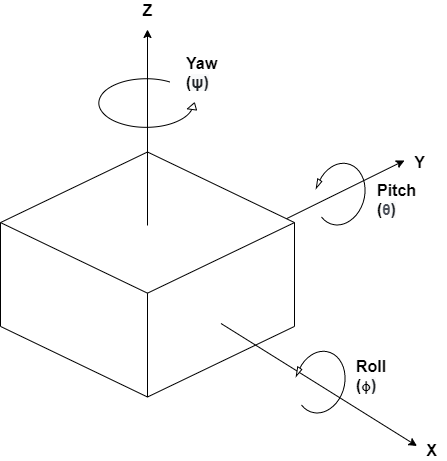
\includegraphics[height=2.5in]{background/body_rotations.png}
\end{figure}

\begin{figure}
    \begin{fitbox}[frametitle=Aside: Notation and Nomenclature for Rotations]
        Bodies on their own typically use the ``x, y, z'' notation that is ubiquitous for the Cartesian coordinate system.
        However, when referring to planetary bodies like the Earth, this nomenclature typically changes to North, East, and Down (NED).
        This occurs because on the surface of a large spherical body, we can assume the local area is a plane tangential to the surface.
        To keep the broader scope in mind, we arbitrarily associate the x-axis with East, the y-axis with North, and the z-axis with Down towards the Earth's core (perpendicular to the surface).

        \caption{Illustration of the difference between the global and local reference frames}
        \labfig{global_frame}
        \centering
        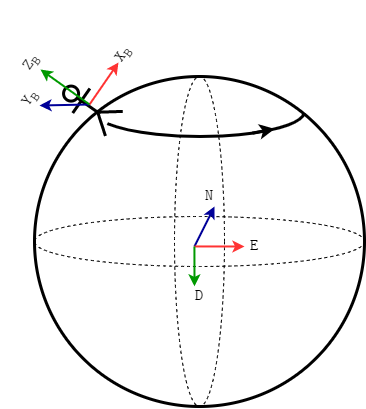
\includegraphics[width=2in]{background/global_frame.png}
    \end{fitbox}
\end{figure}

\subsection{Rotation Matrices} \labsubsec{bkg_orientation_rotation}
A rotation matrix is a mathematical model for translating one body's inertial reference frame to another, e.g. local body to the global body.
These are used for Eulerian transformations of vectors.
The matrix is an $N \times N$ orthogonal matrix where $N$ is the number of dimensions in the vector;
for a three dimensional vector, the rotation matrix to go from one coordinate frame to another would be a $3 \times 3$ matrix.

\begin{figure}[h!]
    \caption[Illustration of rotation between coordinates frame about an axis]{Illustration of the rotation from a base coordinate frame to a local coordinate frame about the axis, $\pmb{r}$}
    \labfig{frame_rotation}
    \centering
    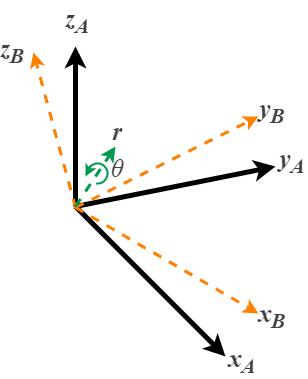
\includegraphics[height=1.75in]{background/frame_rotation.png}
\end{figure}

In Figure \ref{fig:frame_rotation}, we can see a base coordinate frame, $A$, and a different coordinate frame, $B$ that is rotated relative to the base frame about the axis, $\pmb{r}$.
To express the rotation from the base to the local frame, we can borrow notation from Craig \cite{Craig:2022}.
The ``from'' or ``base'' frame is the preceding superscript while the ``to'' or ``local'' frame is the preceding subscript, as shown below:

\begin{equation*}
    {}^A_B R = \left[
        \begin{matrix}
            r_{11} & r_{12} & r_{13} \\
            r_{21} & r_{22} & r_{23} \\
            r_{31} & r_{32} & r_{33}
        \end{matrix}
    \right] = \left[
        \begin{matrix}
            {}^A_Bx & {}^A_By & {}^A_Bz
        \end{matrix}\right]
\end{equation*}

When we want to rotate a vector between frames, we must choose an order in which to do so.
For example, if we wanted to rotate from frame $A$ to frame $B$ using a yaw-pitch-roll rotation order, we can construct the following rotation matrix from Appendix \ref{sec:3d_rot_mat}:

\begin{align*}
    {}^A_B R = R_z(\psi) R_y(\theta) R_x(\phi) &= \left[
        \begin{matrix}
            \cos\psi & -\sin\psi & 0 \\
            \sin\psi & \cos\psi & 0 \\
            0 & 0 & 1
        \end{matrix}\right]
        \left[\begin{matrix}
            \cos\theta & 0 & \sin\theta \\
            0 & 1 & 0 \\
            -\sin\theta & 0 & \cos\theta
        \end{matrix}\right]
        \left[\begin{matrix}
            1 & 0 & 0 \\
            0 & \cos\phi & -\sin\phi \\
            0 & \sin\phi & \cos\phi 
        \end{matrix}\right] \\ \\
        &= \left[\begin{matrix}
            \cos\psi\cos\theta & \cos\psi\sin\theta\sin\phi-\sin\psi\cos\theta & \cos\psi\sin\theta\cos\phi+\sin\psi\sin\phi \\
            \sin\psi\cos\theta & \sin\psi\sin\theta\sin\phi+\cos\psi\cos\phi & \sin\psi\sin\theta\cos\phi-\cos\psi\sin\phi \\
            -\sin\theta & \cos\theta\sin\phi & \cos\theta\cos\phi
        \end{matrix}\right]
\end{align*}

Then, we can rotate the vector from $A$ to $B$ via:

\begin{equation*}
    {}^A_B\pmb{v} = {}^A_B R \cdot {}^A\pmb{v}
\end{equation*}

\paragraph*{Gimbal Lock} When two axes become parallel, Eulerian changes to either axis become irrelevant, ergo, the system loses a degree of freedom.
This condition is called ``gimbal lock''.
When in gimbal lock, rotations yield discontinuities that need to be mitigated by changing the rotation order, or moving two or three axes at once.
This can create strange pathways for the body and cause unexpected behavior.
Monitoring for and breaking gimbal lock are also computationally expensive as the program must perform multiple matrix multiplications and then have logic to determine if a) it is in a gimbal lock condition and b) what rotation order would be required to break the condition.

The figure below shows a body's rotation while in gimbal lock. The rotation order is roll-pitch-yaw.
First, it is pitched 90 degrees upwards to align the roll and yaw axes, $\lbrack 0, 90, 0 \rbrack$ (Figure \ref{subfig:ship_009000}).
If we then want it's orientation to be $\lbrack 90, 0, 0 \rbrack$ (Figure \ref{subfig:ship_900000}), the body would be rolled left 90 degrees and pitched down 90 degrees.
However, due to gimbal lock, the body ended up in the orientation $\lbrack 0, 0, 90 \rbrack$ (Figure \ref{subfig:ship_000090})!
To break the gimbal lock and get to the correct orientation, the rotation order would have to be changed to pitch-yaw-roll, or the roll and yaw axes driven simultaneously.

\begin{figure}[h!]
    \centering
    \subfloat[Start: $\lbrack 0, 0, 0\rbrack$]{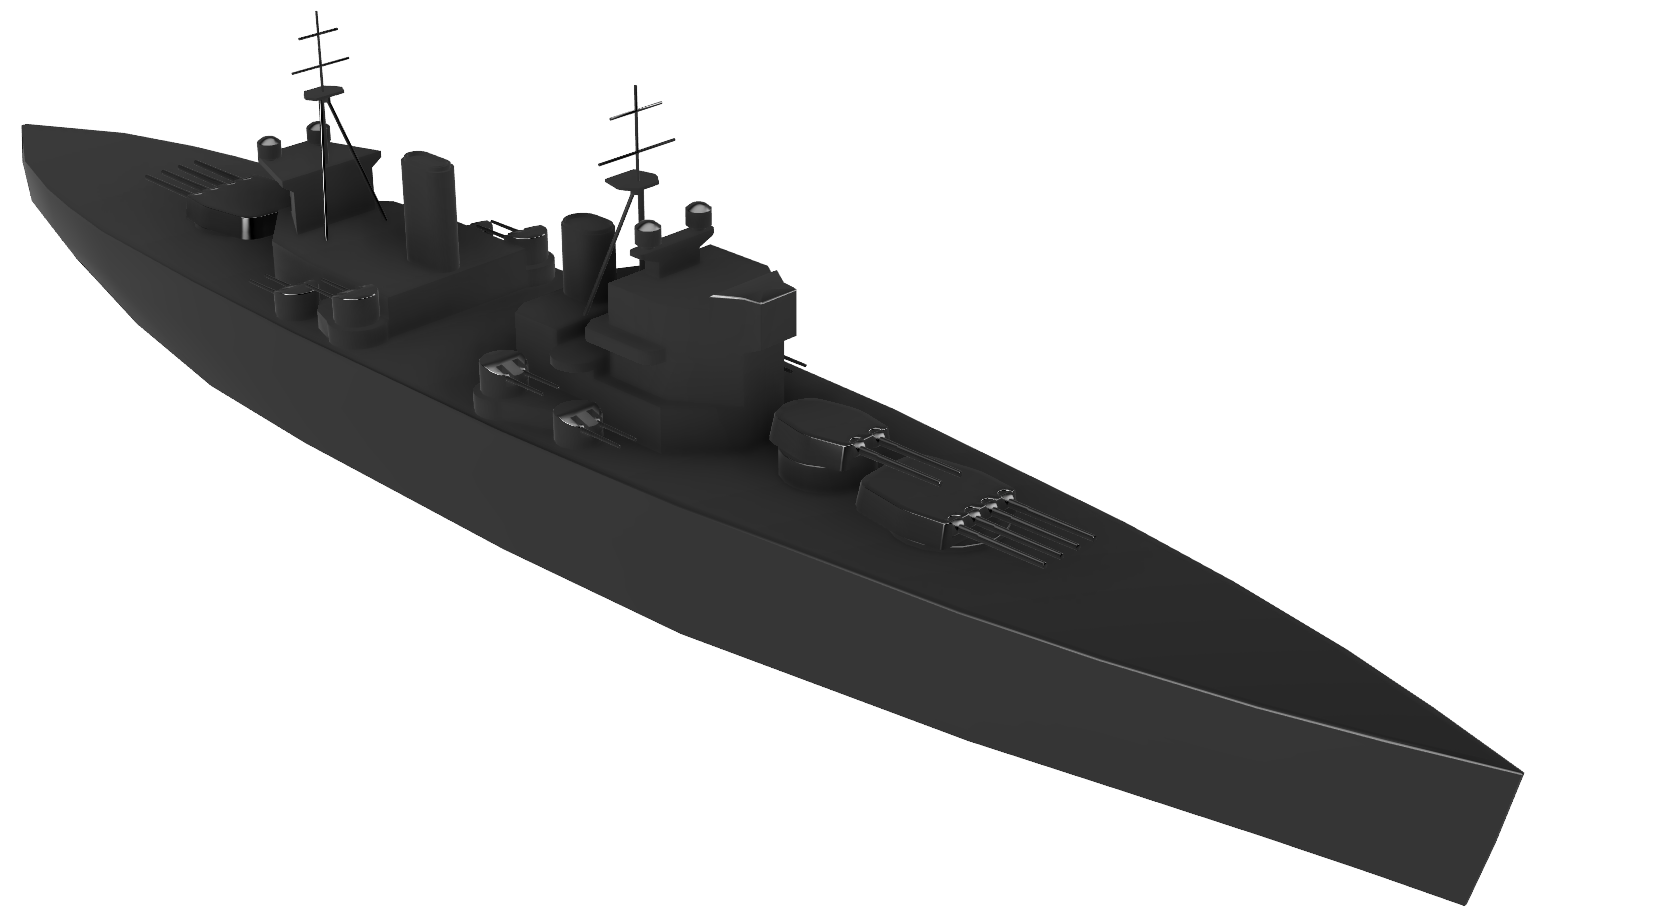
\includegraphics[width=0.25\textwidth]{background/ship_000000}\label{subfig:ship_000000}}\hskip3ex
    \subfloat[$\lbrack 0, 90, 0 \rbrack$]{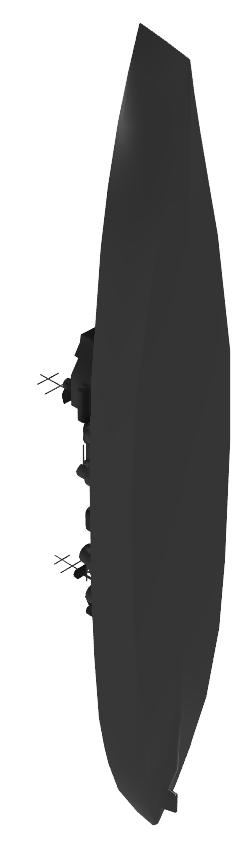
\includegraphics[height=1in]{background/ship_009000}\label{subfig:ship_009000}}\hskip10ex
    \subfloat[$\lbrack 90, 90, 0 \rbrack$]{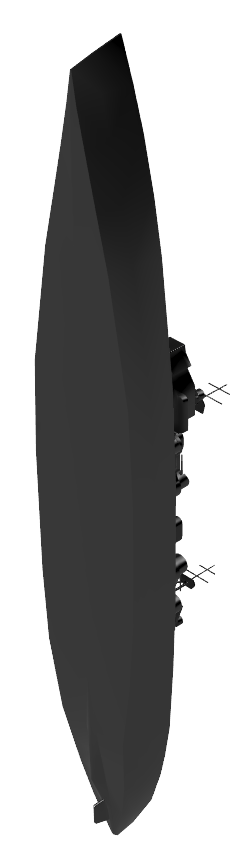
\includegraphics[height=1in]{background/ship_909000}\label{subfig:ship_909000}}\hskip5ex
    \subfloat[End: $\lbrack 0, 0, 90 \rbrack$]{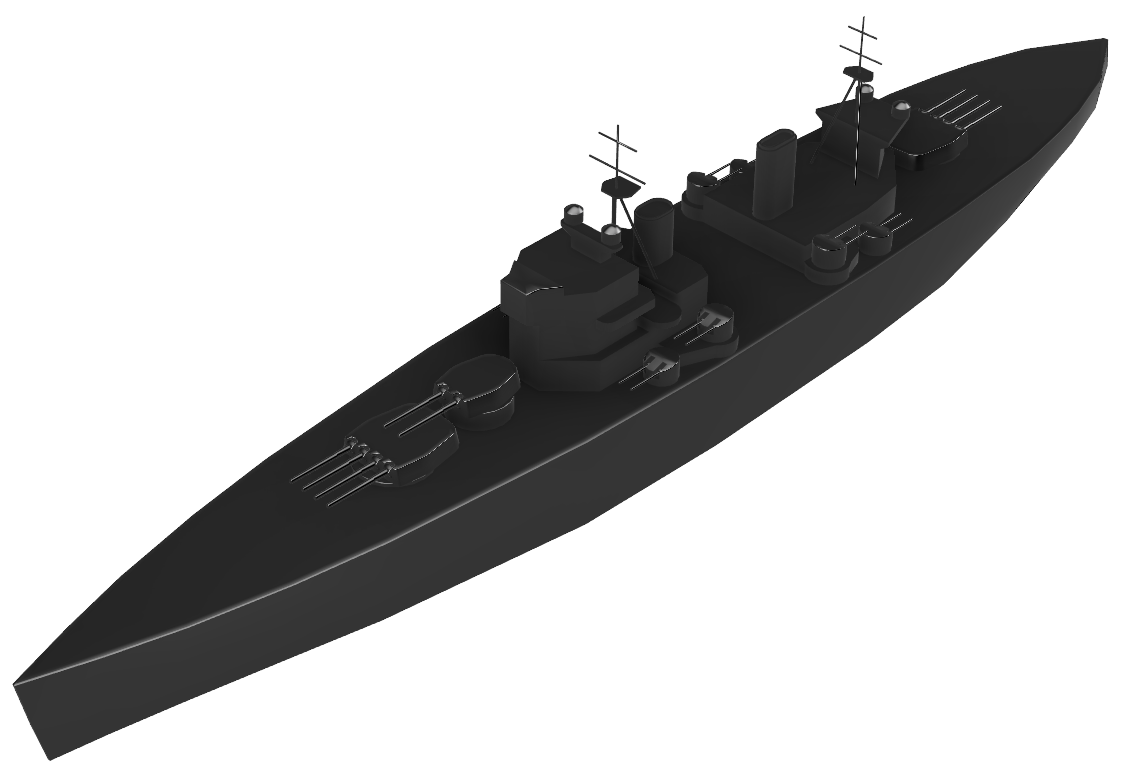
\includegraphics[width=0.25\textwidth]{background/ship_000090}\label{subfig:ship_000090}}
    \subfloat[Desired: $\lbrack 90, 0, 0 \rbrack$]{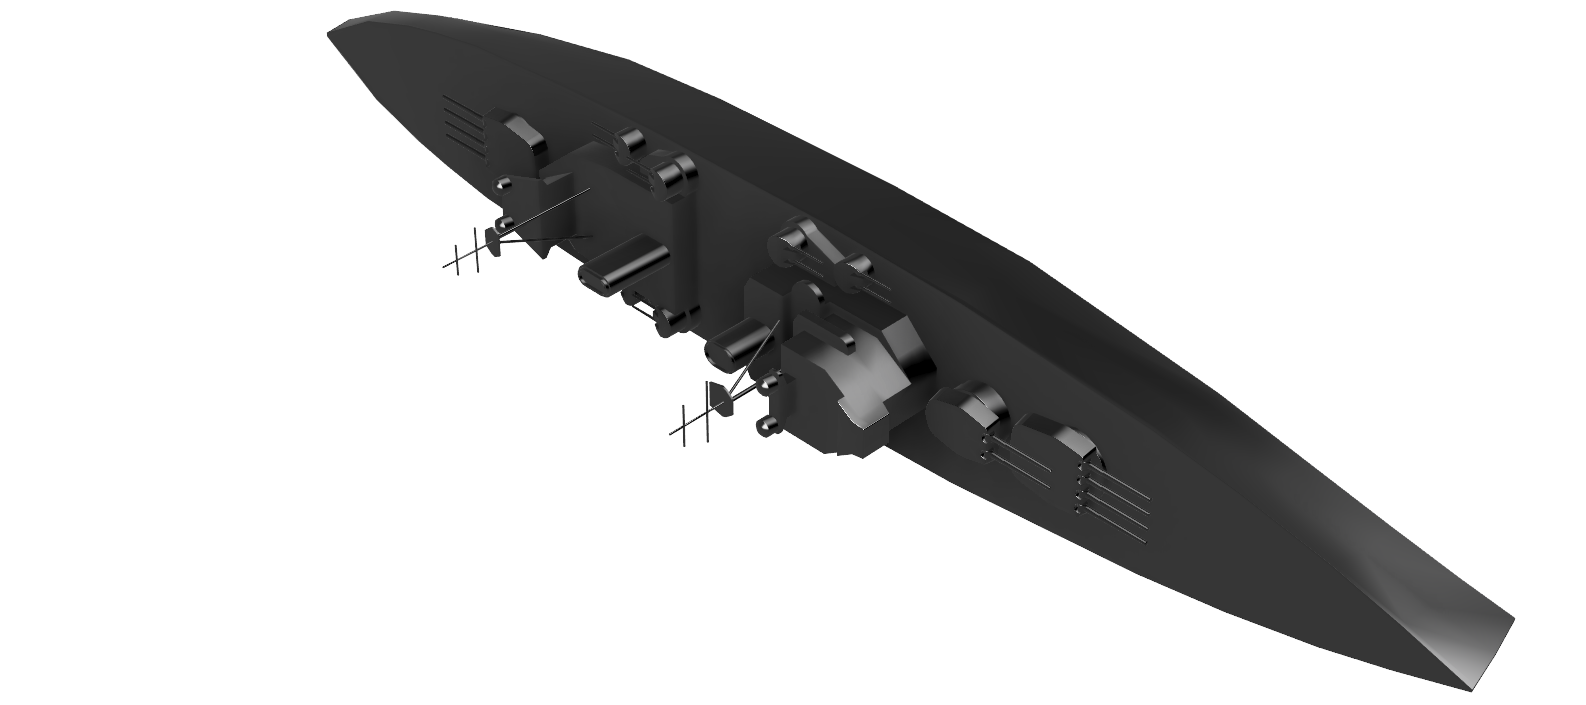
\includegraphics[width=0.25\textwidth]{background/ship_900000}\label{subfig:ship_900000}}
    \caption[Gimbal lock demonstration]{Demonstration of gimbal lock on a rotating 3D body.
    Despite only pitching and rolling the body, the end result of the transformation is an effective yaw.
    This is because the first pitch aligns the roll and yaw axes, effectively making them the same.
    In the given rotation order, any roll rotation would be equivalent to a yaw rotation when the object is pitched 90$^{\circ}$.
    3D model courtesy of ``printable models'' from Free3D.com.}
    \labfig{gimbal_lock}
\end{figure}

\subsection{Quaternions} \labsubsec{quaternions}
In the 19th century, an Irish mathematician was contemplating the problem of Euler angles and analyzing three dimensional geometry.
Sir William Hamilton considered the problem from within the complex or imaginary space and found that a three dimensional vector could not be expressed with a complex triplet.
Instead, Hamilton discovered that the problem could be solved with a complex quadruplet, he called a quaternion \cite{Hamilton:1850}, which could be used as a more mathematically pure tool to understand three dimensional geometry.
For more detailed notes, see Kuipers \cite{Kuipers:2002}

A quaternion exists in four dimensional Hamiltonian space and has three complex and one real component in its vector. 
Like a rotation matrix, it describes the rotation from one reference frame to another about some axis, $\pmb{r}$, as shown in Figure \ref{fig:frame_rotation}.
But, the quaternion is not susceptible to gimbal lock as when two of its axes align, it still retains three degrees of freedom.
Additionally, it is not limited to the range of 0 to 360 (or -180 to 180) like Euler angles and therefore has no discontinuities when looping from one end of the range to the other.
We can express the quaternion from frame $A$ to frame $B$ as:

\begin{equation}
    {}^A_B \pmb{q} =
    \begin{bmatrix}
        q_1 & q_2 & q_3 & q_4
    \end{bmatrix} = 
    \begin{bmatrix}
        w & x & y & z
    \end{bmatrix} = 
    w + x\hat{i} + y\hat{j} + z\hat{k}
\end{equation}

Since the quaternion is just a vector, this drastically simplifies any rotation calculations and improves computational performance.
In order to rotate a vector using a quaternion, we need to set the quaternion to be a unit quaternion by:

\begin{equation}
    \pmb{q} = \frac{\pmb{q}}{\lVert\pmb{q}\rVert}
\end{equation}

Then, we can calculate the inverse quaternion, ${\pmb{q}}^{-1}$ (or conjugate $\pmb{q}^*=\pmb{q}^{-1}, \text{ if } \lVert\pmb{q}\rVert=1)$, using:

\begin{equation}
    \pmb{q}^{-1} = \frac{q_1 - q_2\hat{i} - q_3\hat{j} - q_4\hat{k}}{\lVert\pmb{q}\rVert^2}
\end{equation}

Then, we can rotate a three dimensional vector,${}^A\pmb{v}$, using the equation:

\begin{equation}
    {}^A_B \pmb{v} = {}^A_B\pmb{q} \hspace{0.25em} {}^A\pmb{v} \hspace{0.25em} {}^A_B\pmb{q}^{-1}
\end{equation}

In an inertial measurement unit or attitude and heading reference system, we will need to rotate freely between readings taken in the body's local frame to that in the global frame, e.g. when calculating linear acceleration.
Using the quaternion method above simplifies the calculation and can allow us to more easily determine body attitude from measurements.

\section{Sensing} \labsec{sensing}
Now that we have a basic understanding of some of the mathematical relationships present in inertial tracking, we need to start sensing our environment.
So, how can we compute the position, velocity, acceleration, and attitude of a body in space?
In order to answer this question, we must first examine the different sensors that are available.

\subsection{Magnetometer} \labsubsec{magnetometer}
Magnetometers use magnetoresistive elements that change their effective resistance in the presence of a magnetic field \cite{Corke:2011}.
Atoms within a magnetoresistive element change their orientations with the local magnetic field.
The new orientation can hinder or aid the path of free electrons moving through the element, thus changing the resistance.
By measuring this value and correlating it to a measurement scale, the local strength and direction of a magnetic field can be determined.

\begin{figure}[h!]
    \caption[Magnetometer block diagram]{Basic block diagram of a single-axis magnetometer where electrons are flowing through the magnetoresistive material. The left diagram shows the condition when the magnetic field is aligned (minimal resistance); the right shows the non-aligned magnetic field condition which increases the resistance the electrons face passing through the material.}
    \labfig{magnetometer}
    \centering
    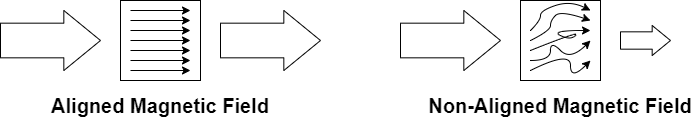
\includegraphics[width=4.5in]{background/magnetometer.png}
\end{figure}

\subsection{Gyroscope} \labsubsec{gyroscope}
A gyroscope is an inertial sensor that measures the angular velocity of a rotating body.
MEMS-based gyroscopes measure this value by applying the Coriolis effect on a microscopic mass \cite{Corke:2011}.
As shown in Figure \ref{fig:gyroscopes}, an oscillation is induced on the x-axis using a driving circuit.
While oscillating, if an angular velocity ($\omega$) is imparted on the z-axis, the suspended mass will experience a force in the y-axis that is proportional to $\omega$ (Appendix \ref{chap:gyroscope_proof}).
Newton's Second Law can be applied to directly correlate the force experienced to a displacement and therefore a change in resistance or capacitance.

\begin{figure}[h!]
    \caption[Gyroscope block diagram]{Basic block diagram of a three-axis gyroscope where the masses are suspended from springs. The left diagram shows a single mass configuration; the right shows a tuning fork configuration which is twice as sensitive as the singular mass.}
    \labfig{gyroscopes}
    \centering
    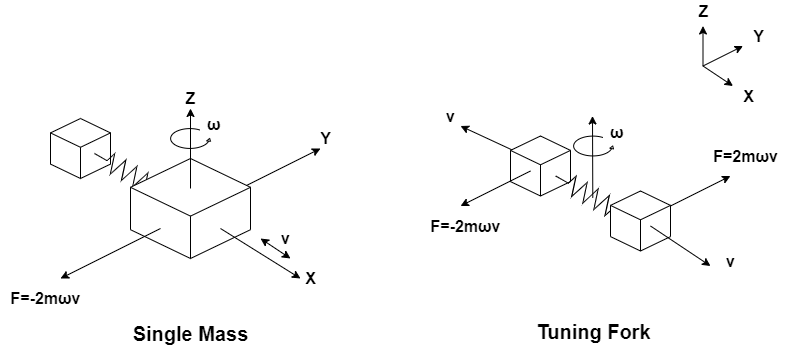
\includegraphics[width=4.5in]{background/gyroscopes.png}
\end{figure}

\subsection{Accelerometer} \labsubsec{accelerometer}
Accelerometers measure a change in velocity over time (acceleration).
An accelerometer is comprised of a mass suspended in an axis of motion by springs of a known K-constant \cite{Corke:2011}.
From Newton's Second Law as applied to a spring-mass system, $\frac{-K}{m}x=a$, we can directly correlate the displacement of the mass to the magnitude of the acceleration along the measurement axis.
Typically, this scale is electrically resistive or capacitative and creates an analog change in a driving (exciting) voltage which can be measured in a circuit using a Wheatstone Bridge (Appendix \ref{chap:wheatstone_bridge}) and microcontroller.
A basic representation of a three-axis accelerometer is shown in Figure \ref{fig:accelerometers}.

\begin{figure}[h!]
    \caption[Accelerometer block diagram]{Basic block diagram of a three-axis accelerometer where the masses are suspended from springs.}
    \labfig{accelerometers}
    \centering
    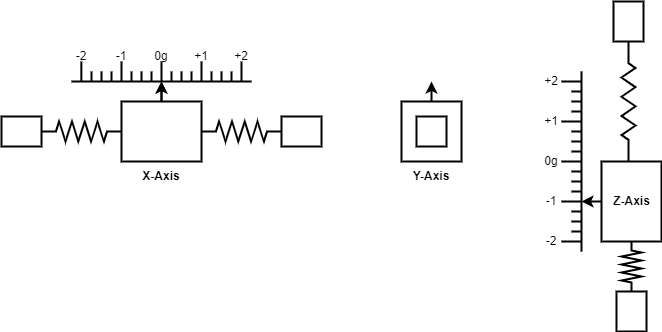
\includegraphics[width=4.5in]{background/accelerometers.png}
\end{figure}

\subsection{MARG Arrays and Inertial Measurement Units} \labsubsec{marg_imu}
Now, with the basics of each sensor in mind, we can combine them into a single package, called a Magnetic, Angular Rate, and Gravity (MARG) array.
Each of the above diagrams represent a single sensing axis, or Degree of Freedom (DOF).
In order for a MARG array to be useful in a 3D environment, it needs to have three sensing axes orthogonal to each other.
Each DOF will measure the x-, y-, and z-axis, respectively with the positive sensing direction according to the right hand rule.
By combining multiple tri-axial arrays, we can define different types of Inertial Measurement Units (IMUs), as shown in Table \ref{tab:imu_dofs}.
Typically, the more sensing axes, the more accurate the array will be (depending on the performance of the sensor fusion algorithm).
Note that a MARG array is an IMU with an integrated tri-axial magnetometer .

\begin{table}[h]
    \caption{Common definitions for IMUs of varying degrees of freedom.}
    \labtab{imu_dofs}
    \centering
    \begin{tabular}{| c | c | c | c | c |}
        \hline
        DOFs & Accelerometer & Gyroscope & Magnetometer & Barometer \\
        \hline
        3-DOF & 3-axis\tablefootnote{can be either or, but not both.} & 3-axis\footnotemark[\value{footnote}] & --- & --- \\
        6-DOF & 3-axis & 3-axis & --- & --- \\
        9-DOF & 3-axis & 3-axis & 3-axis & --- \\
        10-DOF & 3-axis & 3-axis & 3-axis & 1-axis \\
        \hline
    \end{tabular}
\end{table}

\begin{figure}
    \begin{fitbox}[frametitle=Aside: MEMS Technology]
        During the Apollo program, the ST124-M inertial measurement unit was developed that fed the Saturn V rocket's inertial characteristics to the main flight computer \cite{Thomason:1965}.
        The IMU consisted of a tri-axial gyroscope array, redundant tri-axial accelerometer arrays, pendulums, and other sensors.
        While it was a technological marvel at the time, it was the size of a basketball and weighed about 45-65 kilograms.
        Modern cellphones with the same capability are orders of magnitude smaller, lighter, and cheaper; so, what happened?

        \begin{center}
            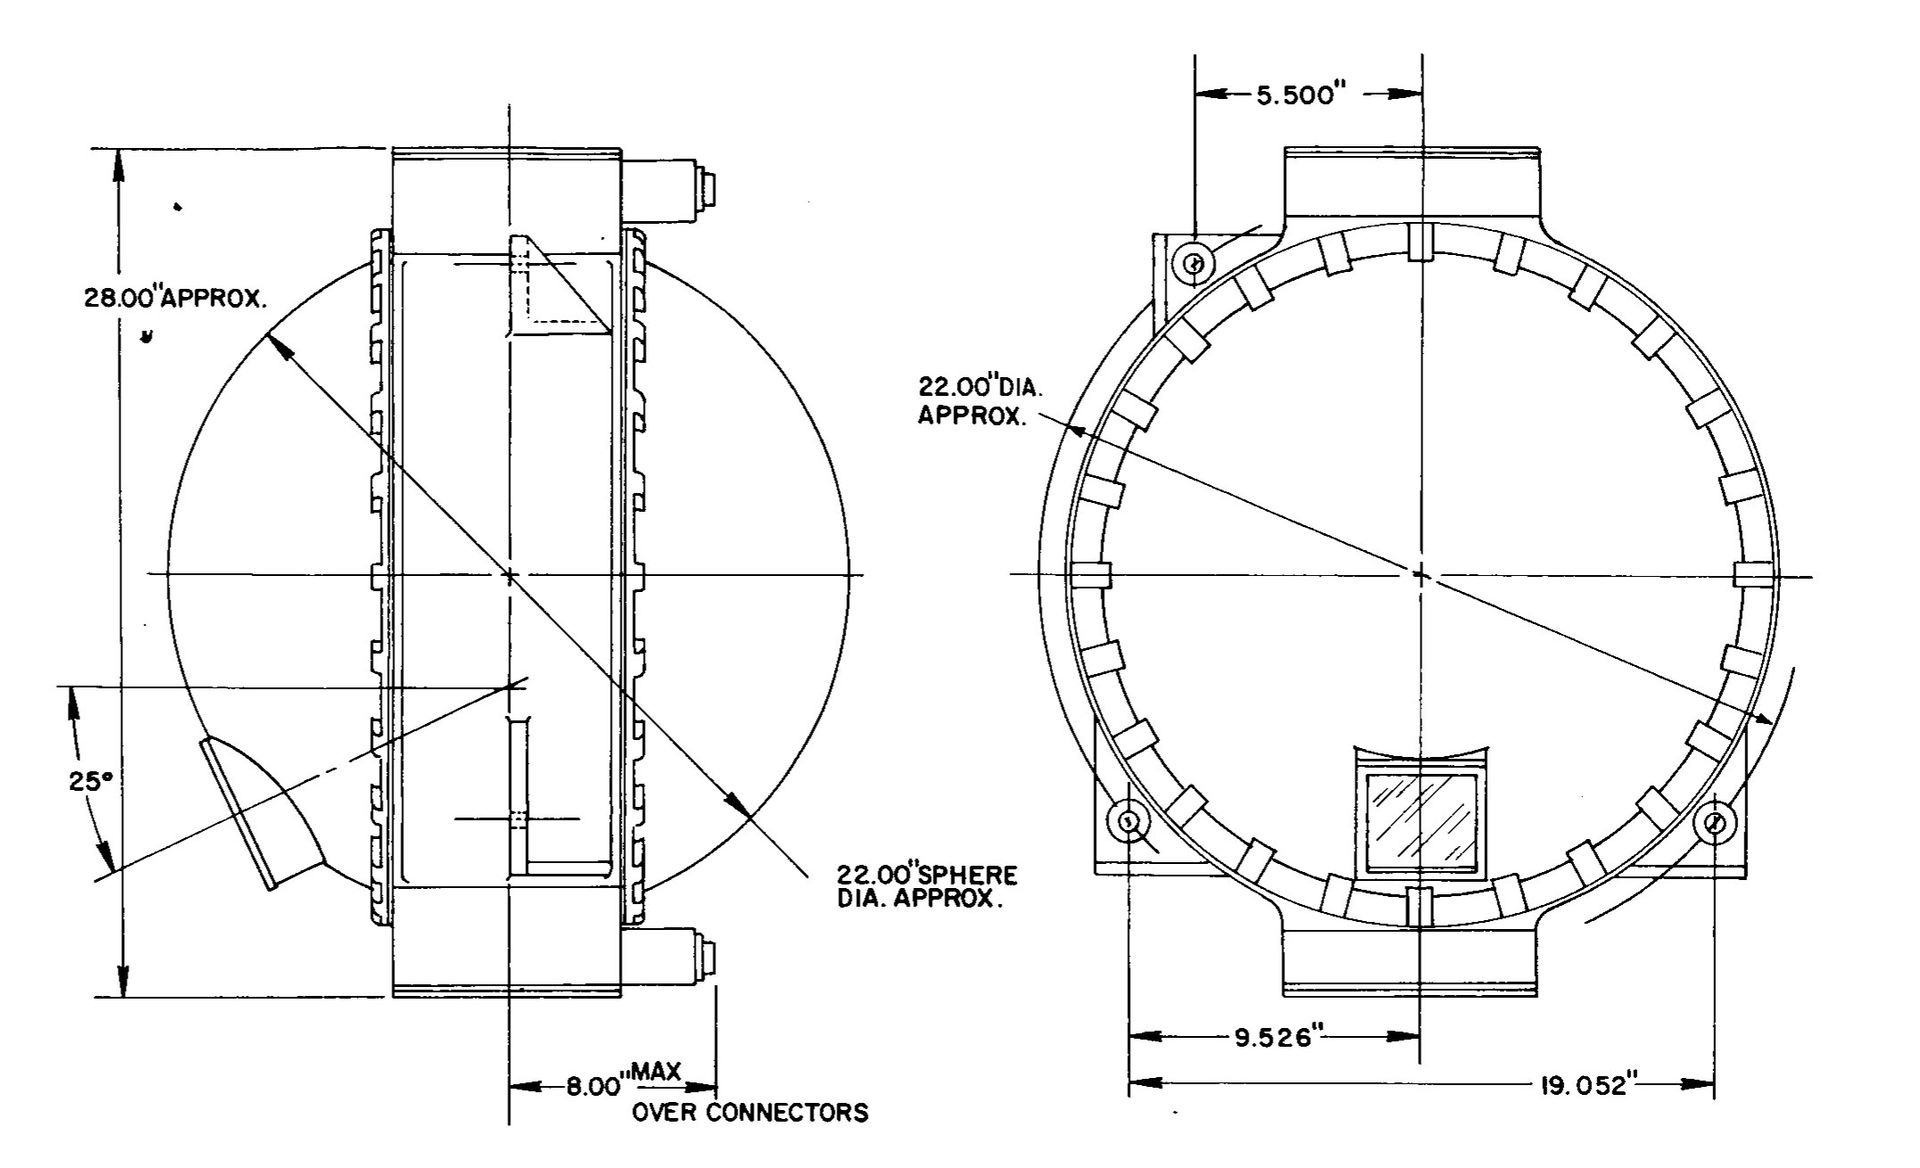
\includegraphics[height=3in]{images/background/Apollo_IMU_exhibit.jpg}
            % \caption[Test]{ST124-M inertial measurement unit courtesy of NASA \url{https://en.wikipedia.org/wiki/ST-124-M3_inertial_platform#/media/File:ST124-M_drawing.jpg}}
            \caption[ST124-M Outline]{ST124-M inertial measurement unit courtesy of NASA \cite{Thomason:1965}}
        \end{center}

        Modern manufacturing methods have enabled a new technology called Microelectromechanical Systems, or MEMS.
        MEMS are microscopic devices that perform an electromechanical function such as sensing acceleration, rotation rate, or magnetic fields \cite{MEMS:2023}.
        They are the most common technology in modern sensor development and revolutionized the technology space by shrinking components down to the micro- and nanometer scales.
        Due to the advent of MEMS technology, devices such as accelerometers, magnetometers, gyroscopes, barometers, hygrometers, etc. have been shrunk down from large mechanical masterpieces to mass-producible products that fit within a few square millimeters of epoxy.
        This dramatically cheapened these devices and has allowed more products to integrate smart sensors into their designs.
    \end{fitbox}
\end{figure}

According to VectorNav \cite{VectorNav:2023}, a producer of industrial-grade IMUS, the cheapest, least precise, and least accurate IMUs are considered ``consumer-grade''.
Every day smartphones, cheap commercial breakout boards, and even shipping crates have these devices on-board.
Consumer-grade IMUs can be bought for cents, dollars, or tens of dollars per unit in bulk and are ideal for mass production spaces where quantity is king over quality.
A step up from these sensors are ``industrial-grade'' IMUs. 
These are tens to hundreds of dollars per unit but are an order of magnitude more accurate and precise than their consumer counter parts.
This makes them desirable for the automotive and industrial sectors as they can assist in automation, control, and monitoring of expensive unmanned systems.
The ``tactical-grade'' sensors are even more robust and accurate than the previous tiers and have an appropriate military-industrial complex price tag to match. 
These devices will typically be used in applications where war fighters need precise guidance for munitions, or need to navigate their way through hazardous and/or GPS-denied terrain.
Finally, the last major tier are the ``navigation-grade'' sensors. 
These sensors are extremely precise, extremely accurate, and cost more than some middle-class families will make in a year.
Primarily, these will be used in survey missions or on underwater vehicles where absolute precision and knowledge of their location is necessary.

\subsection{Global Positioning System} \labsubsec{gps}
The Global Position System, or GPS, is a constellation of high-altitude satellites that service most of the globe \cite{Hofmann:2001}.
First developed by the US military for large scale maneuvers on the battlefield, GPS is a ubiquitous technology that is available in almost every device from smartphones to cars.
Each GPS satellite in orbit transmits the current time measured by their internal atomic clocks.
A GPS receiver on the ground can synchronize its own internal clock to the GPS time and wait for a satellite's transmission.
When the satellite time is received, the device can determine the difference between its clock and the satellite's report called the Time of Flight (ToF).
Since the Time of Flight can be assumed to be the constant speed of light, the GPS receiver can determine its distance to a satellite in a known orbit.
Repeat for at least three satellites, and a GPS receiver can triangulate its position to a reasonable circle of error of about 3-meters.

\begin{figure}[h!]
    \caption[GPS diagram]{Basic representation of how GPS communicates with a device to calculate its position on Earth.
    GPS satellites in orbit broadcast a time and using trigonometry and algebra, a device can calculate the distance to various satellites and triangulate its position.}
    \labfig{gps}
    \centering
    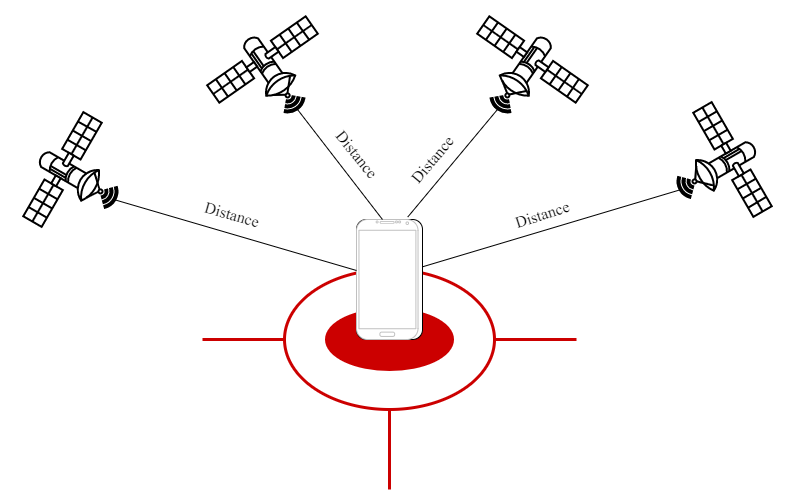
\includegraphics[width=4.5in]{background/gps.png}
\end{figure}

\section{Sensor Fusion} \labsec{sensor_fusion}
While having each individual sensor will give some data, they offer an incomplete picture of a body's orientation and movement through space.
An accelerometer can detect acceleration and determine pitch and roll using basic vector math, but it cannot determine yaw or heading.
Data from a gyroscope can be integrated over time to determine the sensor's attitude, but this method will drift over time and accumulate errors, it also cannot detect movement.
Magnetometers in a weak magnetic field, like Earth's, are not accurate enough to determine roll and pitch, but can easily provide heading.
Finally, GPS readings will provide position and velocity vectors, but typically update slowly and have a large circle of error and cannot determine attitude.
To make these sensors more effective for an inertial sensing application, we need to fuse the data feeds into a unified output that emphasizes the strength of each sensor, while mitigating their limitations.

\subsection{Attitude and Heading Reference System} \labsubsec{ahrs}
An Attitude and Heading Reference System (AHRS) is an IMU equipped with an accelerometer, gyroscope, and/or a magnetometer in all three axes.
The data streams from the sensors can be fused together with external information like GPS data and mathematical models to estimate a body's inertial orientation in three dimensional space.
The block diagram for this operation is shown in Figure \ref{fig:ahrs_design}.
Many algorithms exist to do this sensor fusion such as the the Fast Complimentary Filter \cite{FCF:2016}, Kalman filter \cite{Kalman:1960}, the Mahony filter \cite{Mahony:2008}, and the Madgwick filter \cite{Madgwick:dissertation}.

\begin{figure}[h!]
    \caption[AHRS block diagram]{Basic block diagram of an AHRS. 
    The acceleration, rotation rates, and magnetic field readings are fused together in the IMU the filtered using calibration data. 
    The AHRS can then apply a bias from the GPS course and corrections from a mathematical model of the system.}
    \labfig{ahrs_design}
    \centering
    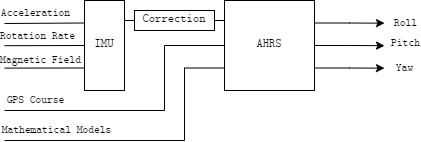
\includegraphics[height=1.3in]{background/ahrs.png}
\end{figure}

Before measurements are fed into a sensor fusion algorithm, the data should be pre-filtered based on known calibration data.
This will improve the sensor fusion performance and accuracy of the resultant values.

\subsection{Inertial Calibration}

From Madgwick \cite{Madgwick:dissertation}, in order to calibrate an IMU, we first need to create a model of the data. For the accelerometer and gyroscope, we can create an inertial model defined as:

\begin{gather} \labeq{inertial_model}
    \pmb{i}_c=MS(\pmb{i}_u-\pmb{b}) \\
    \begin{aligned}
        \text{where } & \pmb{i}_C \text{ is the calibrated inertial measurements,} \\ 
        & M \text{ is the misalignment matrix,} \\
        & S \text{ is the sensitivity identity matrix,} \\
        & \pmb{i}_u \text{ is the uncalibrated inertial measurements, and} \\
        & \pmb{b} \text{ is the bias or offset vector}
    \end{aligned} \notag
\end{gather}

The three calibration values, $M$, $S$, and $\pmb{b}$, represent a set of correction factors that make the measured values more accurate. The inertial measurement is generalized here to represent either accelerometer or gyroscope data. Each sensor will have its own set of the calibration values.

\paragraph*{Bias Vector} The bias, or offset, vector is the average of the inertial readings while the sensor is in a stable, known orientation. For example, when the gyroscope is at rest, we would expect the measurement output to be $\lbrack 0,0,0 \rbrack$ [deg/sec]. However, we may measure an average of $\lbrack 0.89, -0.66, 0.31 \rbrack$ [deg/sec] instead. By subtracting this bias vector from the measurements, we eliminate any unintentional offset from our readings. The bias can be calculated using the equation below:

\begin{gather} \labeq{gyroscope_bias}
    \pmb{b}_g = \frac{1}{N} \sum_{n=0}^N{\pmb{g}_n} \\
    \begin{aligned}
        \text{where } & \pmb{b}_g \text{ is the bias vector,} \\
        & N \text{ is the number of collected samples to average, and} \\
        & \pmb{g}_n \text{ is the uncalibrated gyroscope measurement vector}
    \end{aligned} \notag
\end{gather}

For accelerometers, the bias is calculated differently. Each measurement axis must be exposed to ±1g of acceleration by placing the instrument vertical on each of the measurement axes in both the positive and negative directions. The bias for each axis can then be determined by taking the average value as shown below:

\begin{gather} \labeq{accelerometer_bias}
    b_a = \frac{1}{2} \left[ \frac{1}{N}\sum_{n=0}^N{a_{n,+g}} + \frac{1}{M}\sum_{m=0}^M{a_{m,-g}} \right] \\\
    \begin{aligned}
        \text{where } & b_a \text{ is the bias for a measurement axis,} \\
        & N \text{ is the number of samples taken in the +1g orientation,} \\
        & a_{+g} \text{ is the average axis measurement when exposed to +1g,}\\
        & M \text{ is the number of samples taken in the -1g orientation, and} \\
        & a_{-g} \text{ is the average axis measurement when exposed to -1g}
    \end{aligned} \notag
\end{gather}

\paragraph*{Sensitivity Matrix} The sensitivity matrix is a diagonal matrix that accounts for minor errors with variations in manufacturing process and sensor material. 
These errors can make each uniaxial sensor in a triaxial array sense the environment slightly differently. 
While bias covers this area when at rest or in specific orientations, the sensitivity error will change depending on the motion and orientation. 
To account for this, we need to expose each sensor to a known reference stimulus and calculate the sensitivity based on the average magnitude of the measurement vector during that time. 
For a gyroscope, this value can be an arbitrary, but constant, rotation rate, $\omega$. 
For an accelerometer, this value will be ±1g. The equations for each gyroscope and accelerometer axis are provided below:

\begin{gather} \labeq{gyroscope_sensitivity}
    s_{g, \omega} = \frac{\lVert g_{+\omega}\rVert + \lVert g_{-\omega}\rVert}{2\omega} \\
    \begin{aligned}
        \text{where } & s_{g,\omega} \text{ is the sensitivity value for each gyroscope axis when exposed to } \omega , \\
        & g_{+\omega } \text{ is the average gyroscope axis reading whe exposed to +} \omega ,\\
        & g_{-\omega } \text{ is the average gyroscope axis reading whe exposed to -} \omega , \text{ and} \\
        & \omega \text{ is the reference rotation rate}
    \end{aligned} \notag
\end{gather}

\begin{gather} \labeq{accelerometer_sensitivity}
    s_{a, g} = \frac{\lVert a_{+g} \rVert + \lVert a_{-g} \rVert}{2} \\
    \begin{aligned}
        \text{where } & s_{a,g} \text{ is the sensitivity value for each axis when exposed to 1g,} \\
        & a_{+g} \text{ is the average axis measurement when exposed to +1g, and} \\
        & a_{-g} \text{ is the average axis measurement when exposed to -1g}
    \end{aligned} \notag
\end{gather}

After calculating these values for each axis, we can form the sensitivity matrix for the gyroscope and accelerometer like so:

\begin{equation}
    S_g = 
    \begin{bmatrix}
        s_{g,x} & 0 & 0 \\
        0 & s_{g,y} & 0 \\
        0 & 0 & s_{g,z}
    \end{bmatrix} 
\end{equation}
\begin{equation}
    S_a =
    \begin{bmatrix}
        s_{a,x} & 0 & 0 \\
        0 & s_{a,y} & 0 \\
        0 & 0 & s_{a,z}
    \end{bmatrix}
\end{equation}

While this calibration value accounts for some of the intrinsic sensor error, it does not account for axes misalignment or non-orthogonality within the sensor. To accomplish this, we must incorporate the misalignment matrix.

\paragraph*{Misalignment Matrix} The misalignment matrix is the final, but most complex, calibration value that we can calculate for the inertial sensors. It reduces error from multiple sources such as non-orthogonality between the measurement axes, the misalignment from the measurement axes to the actual sensor packaging, and misalignment from the package onto the application board. In order to calculate the misalignment matrix, we must consider it as the solution to a non-linear problem. First, we must define an objective function for the solution space. Since the goal of the misalignment matrix is to reduce error, then we can define the objective function as the Root Mean Square Error (RMSE) of the measurement vector, the misalignment vector, and the reference vector:

\begin{gather} \labeq{misalignment_obj_func}
    RMSE = \sqrt{\frac{1}{N}\sum_{n=0}^N{\|{\pmb{i}_{n,u} \cdot M^* -\pmb{i}_{n,\text{ref}}\|}^2}} \\
    \begin{aligned}
        \text{where } & N \text{ is the number of samples in the dataset,} \\
        & \pmb{i}_{n,u} \text{ is the uncalibrated measurement vector with the bias removed,} \\
        & M^* \text{ is the guessed $3 \times 3$ matrix that corrects $\pmb{i}_{n,u}$ to be near $\pmb{i}_{\text{ref}}$, and } \\
        & \pmb{i}_{\text{ref}} \text{ is the reference stimulus vector for the measurement}
    \end{aligned} \notag
\end{gather}

Then, given a dataset of measurement vectors and their expected reference vectors, we can use a non-liner solver\footnote{Like the \href{https://docs.scipy.org/doc/scipy/reference/generated/scipy.optimize.minimize.html}{\lstinline{scipy.optimize.minimize} toolbox}} to determine the value of $M^*$ 
Assuming the sensitivity was not removed from the measurement signal, the $M^*$ matrix happens to include it as its diagonal. 
By extracting the diagonal and normalizing the original matrix, we are left with the sensitivity and misalignment matrix calibration values.

\begin{gather} \labeq{sensitivity_and_misalignment}
    S = \text{diag}(M^*) \\
    M = M^* \cdot S^{-1} \notag
\end{gather}

We can now apply the misalignment matrix, sensitivity matrix, and bias vector to the sensor readings according to the model in Equation \ref{eq:inertial_model}. 
This should yield outputs that are close to the real values, which is examined in Chapter \ref{chap:calibration}.

\subsection{Magnetic Calibration}
The magnetometer in a MARG array needs a different sensor model than the inertial sensors because the ambient magnetic field introduces different errors. 
There are two types: soft iron, $W$, and hard iron, $\pmb{v}$. 
A hard iron distortion is introduced by magnetic materials placed near the sensor. 
This can occur when the sensor is placed in a casing with permanent magnets or near a speaker, as shown in Tuupola \cite{Tuupola:2018}. 
Soft iron distortion is typically less severe than hard iron distortion and is caused by materials near the sensor that distort the local magnetic field. 
The soft iron distortion can also account for misalignment and sensitivity errors. 
The sensor model for a calibrated magnetometer is given below:

\begin{gather} \labeq{magnetic_model}
    \pmb{m}_c=W^{-1}(\pmb{m}_u-\pmb{v}) \\
    \begin{aligned}
        \text{where } &\pmb{m}_c \text{ is the calibrated magnetometer vector,} \\
        &W^{-1} \text{ is the inverse soft iron matrix,}\\
        &\pmb{m}_u \text{ is the uncalibrated magnetometer vector,} \\
        &\pmb{v} \text{ is the hard iron bias vector}
    \end{aligned} \notag
\end{gather}

With a calibrated sensor in an ideal environment, we would expect a sphere centered on the origin with a radius equal to the magnitude of the local magnetic field. 
Due to the hard and soft iron distortions, this will rarely be the case. 
Hard iron distortion can be removed from the signal by determining the average of the minimum and maximum values of each axis, as shown below:

\begin{equation} \labeq{hard_iron_offset}
    \pmb{v}=\frac{1}{2}
    \begin{bmatrix}
        \max(m_x)+\min(m_x) \\
        \max(m_y)+\min(m_y) \\
        \max(m_z)+\min(m_z)
    \end{bmatrix}
\end{equation}

Once the hard iron distortion is removed from the signal, we should see the readings more closely adhere to the correct spherical shape. 
Then, we can apply Li’s ellipsoid fitting algorithm \cite{Li:2004} to characterize the fit of the optimal ellipsoid for the data, expressed as the symmetrical matrix, $A$. 
Ozyagcilar \cite{Ozyagcilar:2015} builds a relationship between the ellipsoid fit and the soft iron matrix, summarized by:

\begin{equation} \labeq{soft_iron_matrix}
    W^{-1}=A^{1/2}
\end{equation}

With these calibration parameters calculated, they can be used in a sensor fusion algorithm to increase the accuracy of the magnetometer. 
However, these parameters must be recalibrated whenever the sensor enters a new magnetic environment since either the hard or soft iron distortion could be different than previously calculated.

\begin{figure}
    \centering
    \begin{subfigure}[b]{0.3\textwidth}
        \centering
        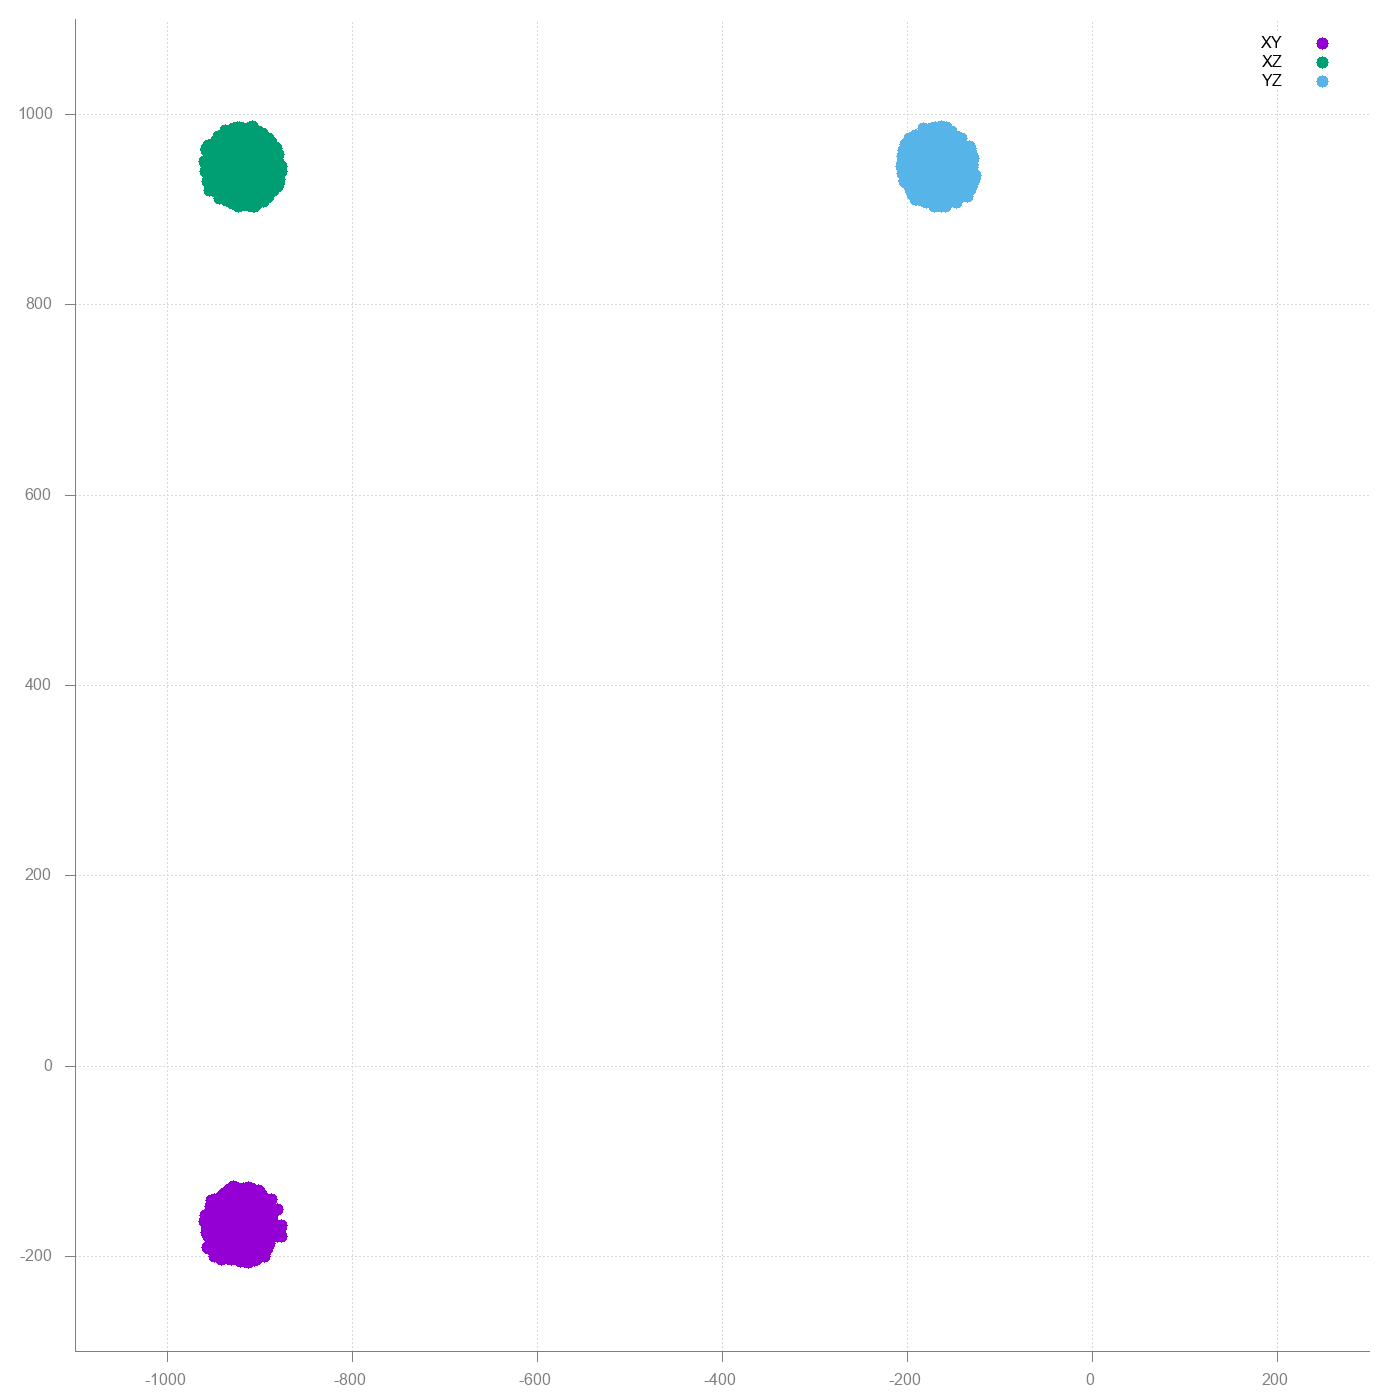
\includegraphics[width=\textwidth]{background/mag_raw.png}
        \caption[Raw Magnetometer Readings]{Example of hard iron distortion from a magnet near a magnetic sensor. Courtesy of Tuupola \cite{Tuupola:2018}.}
        \label{subfig:mag_raw}
    \end{subfigure}
    \hfill
    \begin{subfigure}[b]{0.3\textwidth}
        \centering
        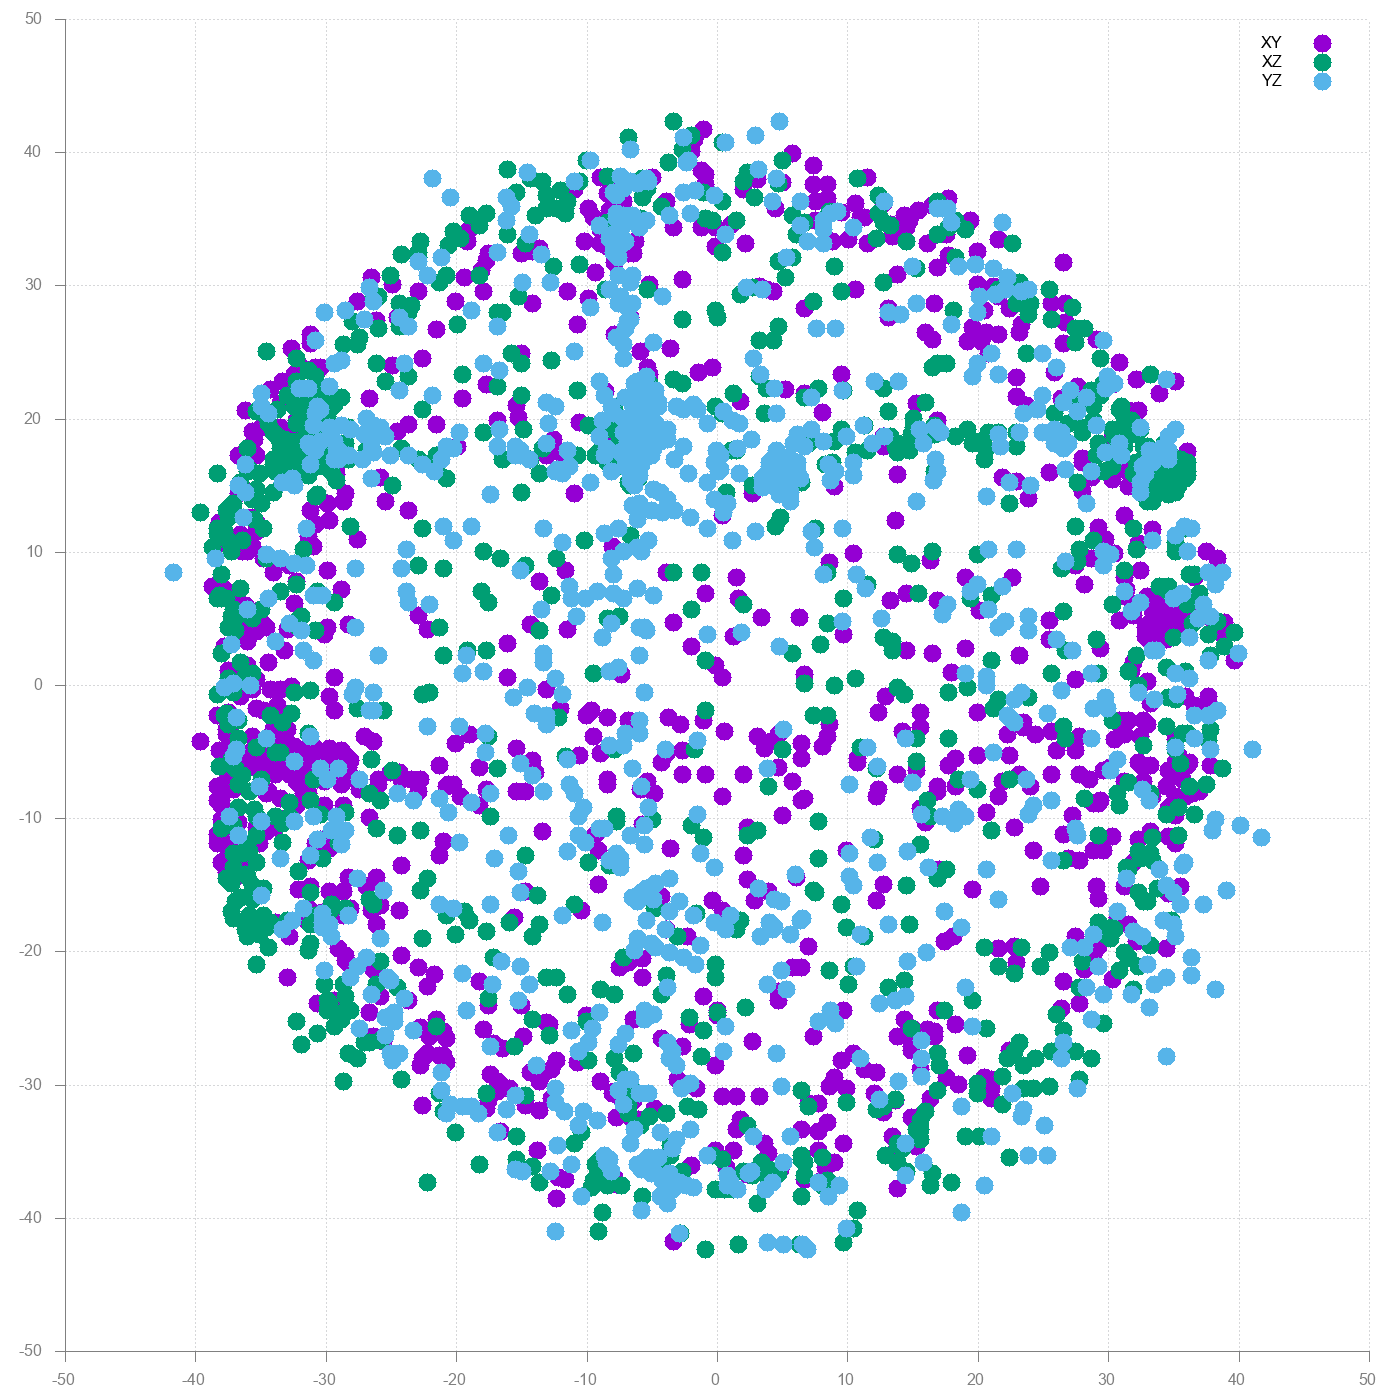
\includegraphics[width=\textwidth]{background/mag_hid.png}
        \caption[Hard Iron Distortion Removed]{Magnetometer calibration data with hard iron distortion removed. Courtesy of Tuupola \cite{Tuupola:2018}}
        \label{subfig:mag_hid}
    \end{subfigure}
    \hfill
    \begin{subfigure}[b]{0.3\textwidth}
        \centering
        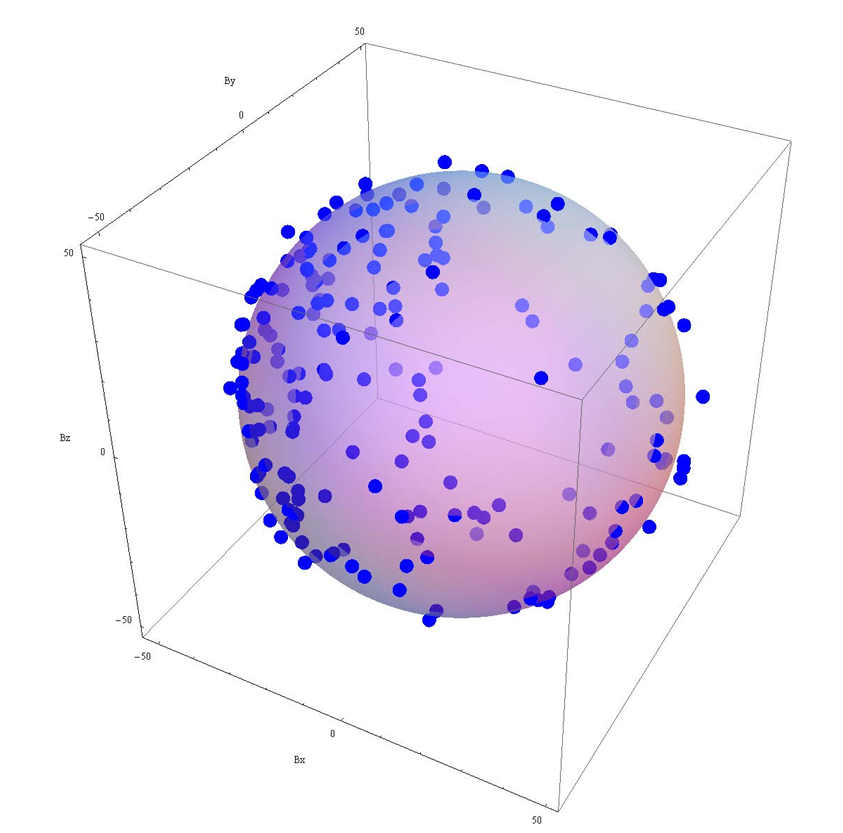
\includegraphics[width=\textwidth]{background/mag_sid.png}
        \caption[Soft Iron Distortion Removed]{Magnetometer calibration data with soft and hard iron distortion removed and fitted to a sphere. Courtesy of Ozyagcilar \cite{Ozyagcilar:2015}}
        \label{subfig:mag_sid}
    \end{subfigure}
       \caption{Correction of magnetic field readings by removing hard and soft iron distortion}
       \labfig{magnetometer_corrections}
\end{figure}

\subsection{Fast Complimentary Filter} \labsubsec{complimentary_filter}
A complimentary filter take advantage of the problems inherent with the accelerometer and gyroscope measurements such they \textit{compliment} each other.
By integrating gyroscopic measurements, we can quickly obtain the body's attitude but the errors in the gyroscope sensor cause this value to quickly drift away from the ``true'' value.
Accelerometer measurements on the other can use trigonometry on the gravitational acceleration vector to determine pitch and roll (tilt).
These measurements are affected by the body's motion and can drift over time as the body experiences other accelerations besides gravity.
An accelerometer also cannot report the yaw rotation, so must be coupled with a tri-axial magnetometer which can also be influenced by external magnetic fields.

In the frequency space, we can consider the gyroscope attitude estimate to drift with a high frequency, and the accelerometer-magnetometer signal to drift with a low frequency.
To compensate for these drifts, we can establish a complimentary or band-pass filter that attenuates the drift signal and outputs the best estimate of orientation.
This filter typically uses a hyperparameter, $\gamma$, to control the attenuation of each of the drifts, i.e. the weight of each estimation like so:

\begin{gather} \labeq{fcf}
    {}^G_B\pmb{q}_{est} = (1-\gamma){}^G_B\pmb{q}_{lf} + \gamma {}^G_B\pmb{q}_{hf} \\
    \begin{aligned}
        \text{where } &{}^G_B\pmb{q}_{est} \text{ is the best estimate of the body quaternion relative to the global frame,} \\
                      &\gamma \text{ is the controlling hyperparameter, } \\
                      &{}^G_B\pmb{q}_{lf} \text{ is the body quaternion estimate from the low frequency drift source, and} \\
                      &{}^G_B\pmb{q}_{hf} \text{ is the body quaternion estimate from the high frequency drift source.}
    \end{aligned} \notag
\end{gather}

Wu et. al \cite{FCF:2016} propose a complimentary filter solution that reports being on par with more computationally expensive fusion algorithms like the Kalman Filter and Madgwick Filter.
This algorithm computes the gravity vector using accelerometer and gyroscope measurements.
By itself, this can yield the tilt attitude of the body.
Then, if there is not severe magnetic distortion detected by the magnetometer, the full attitude can be acquired by fusing together the tilt attitude and that estimated from the magnetometer.
The basic block diagram for the filter is in Figure \ref{fig:fcf_diagram}.

\begin{figure}
    \centering
    \caption[Fast Complimentary Filter]{A simplified block diagram for the Fast Complimentary Filter. 
    Courtesy of Wu et al. \cite{FCF:2016}}
    \labfig{fcf_diagram}
    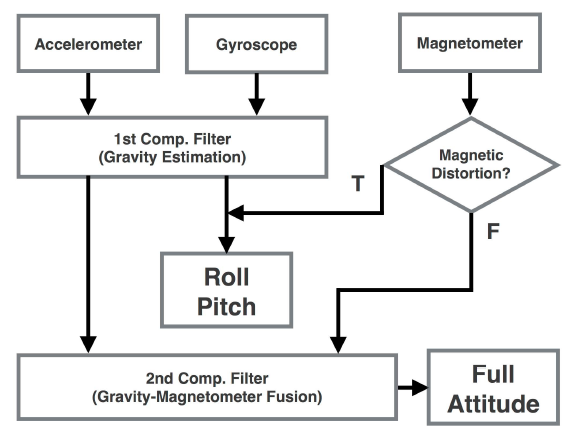
\includegraphics[height=2in]{background/FCF.png}
\end{figure}

\subsection{Kalman Filter} \labsubsec{kalman_filter}
The Kalman Filter \cite{Kalman:1960} was introduced in the 1960's as a method to estimate and track a series of explicit and hidden states within a system.
In a sensor fusion or AHRS application, the Kalman Filter can be used to estimate the orientation state (quaternion) of the system based on the gyroscope, accelerometer, and magnetometer readings.
The Kalman Filter also estimates the uncertainty and noise associated with attitude estimate to give more insightful feedback on the usefulness of the estimate.
At each timestep, the filter uses a built-in mathematical model of the system to predict the current system state and its associated uncertainty.
Then, the filter can predict the state and uncertainty in the next time step and uses that to adjust a correction factor, called the Kalman Gain.
With each iteration of the filter, the Kalman Gain converges on a minimum value and the estimate uncertainty decreases.
The convergence speed and accuracy can be tuned using various hyper parameters like process noise and sensor uncertainty.
The process for the Kalman Filter is shown in Figure \ref{fig:bkg_kalman_filter_process} and a more detailed explanation can be found in Appendix \ref{chap:kalman_filter}.

\begin{figure}
    \centering
    \caption[Kalman Filter Process]{A simplified process block diagram for the Kalman Filter that includes the steps required for each iteration.}
    \labfig{bkg_kalman_filter_process}
    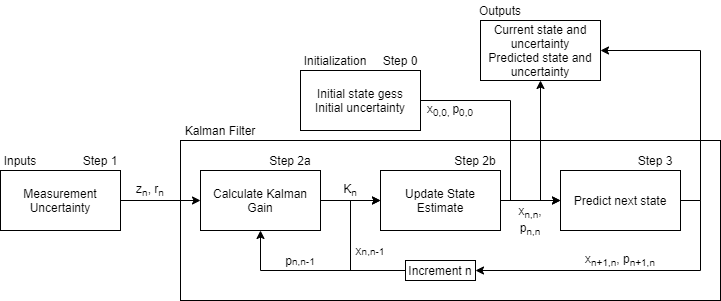
\includegraphics[width=\textwidth]{appendices/kalman-filter/KalmanFilter.png}
\end{figure}

\subsection{Mahony Filter} \labsubsec{mahony_filter}
The Mahony Filter \cite{Mahony:2008} is a deterministic kinematic observer on the Special Orthogonal Group 3 that is driven by instantaneous attitude and angular velocity measurements.
That is, the filter exploits a special relationship between observers to decouple gyroscope measurements from attitude estimates and then does on-line gyroscope bias compensation to increase accuracy.
The filter proposes a model for the gyroscope in the body frame as:

\begin{gather} \labeq{mahony_gyroscope_model}
    \pmb{q} = \pmb{g}_u + \pmb{b}_\omega + \pmb{\mu}_\omega \\
    \begin{aligned}
        \text{where } &\pmb{g} \text{ is the true angular velocity,} \\
                      &\pmb{g}_u \text{ is the uncalibrated measured angular velocity,} \\
                      &\pmb{b}_\omega \text{ is the gyroscope bias vector, and}  \\
                      &\pmb{\mu}_\omega \text{ is the gyroscope measurement noise}
    \end{aligned} \notag
\end{gather}

Additionally, the filter defines the accelerometer measurement as the instantaneous linear acceleration, (i.e. accelerations without the gravitational acceleration vector), with corresponding bias and noise vectors.
The model for the accelerometer is given below:

\begin{gather} \labeq{mahony_accelerometer_model}
    \pmb{a} = {}^G_B R (\pmb{a}_u - \pmb{G}_0 + \pmb{b}_a + )\pmb{\mu}_a \\
    \begin{aligned}
        \text{where } &\pmb{a} \text{ is the true linear acceleration in the body frame,} \\
                      &{}^G_B R \text{ is the rotation matrix from the global to the body frame, } \\
                      &\pmb{G}_0 \text{ is the gravitational acceleration vector,} \\
                      &\pmb{a}_u \text{ is the uncalibrated measured angular velocity, } \\
                      &\pmb{b}_a \text{ is the accelerometer bias vector, and}  \\
                      &\pmb{\mu}_a \text{ is the accelerometer measurement noise}
    \end{aligned} \notag
\end{gather}

These measurements are used to express the body kinematics in an Explicit Complimentary Filter in quaternion form and then rearranged to solve for the change in the body attitude over time, $\pmb{\dot{\hat{q}}}$.
This estimate can be integrated over the sampling time to get the best estimated attitude via:

\begin{gather} \labeq{mahony_filter}
    {}^G_B\pmb{q}_t = {}^G_B\pmb{q}_{t-1} + {}^G_B\pmb{\dot{\hat{q}}}_t \Delta t \\
    \begin{aligned}
        \text{where } &{}^G_B\pmb{q}_t \text{ is the body attitude from the global frame to the local frame at time, $t$,} \\
                      &{}^G_B\pmb{\dot{\hat{q}}}_t \text{ is the time rate of change for the body attitude at time, $t$, and } \\
                      &\Delta t \text{ is the sample interval}
    \end{aligned} \notag
\end{gather}

\subsection{Madgwick Filter} \labsubsec{madgwick_filter}
The Madgwick Filter \cite{Madgwick:dissertation} considers body attitude as an optimization problem that can be solved by a gradient descent algorithm (GDA).
The filter tries to optimize the difference (deviation) between a predefined reference vector in the global frame, ${}^G\pmb{v} = [0, v_x, v_y, v_z]$ with its corresponding measurement vector in the local frame, ${}^B\pmb{s} = [0, s_x, s_y, s_z]$.
This deviation is expressed in the objective function:

\begin{equation} \labeq{madgwick_obj_func}
    f(\pmb{q}, {}^G\pmb{v}, {}^B\pmb{s}) = \pmb{q} \hspace{0.25em} {}^G\pmb{v} \hspace{0.25em} \pmb{q}^{-1} - {}^B\pmb{s}
\end{equation}

The GDA can compute the solution to the objective function by utilizing an initial guess, ${}^G_B \pmb{q}_0$ and a step-size, $\mu$.
This yields the estimate for the quaternion gradient, $\pmb{q}_{\nabla,t}$.
The filter then calculates the time rate of change in the body quaternion, $\pmb{\dot{q}}_t$, as measured from the gyroscopes, $\pmb{q}_{\omega,t}$.
By removing the gyroscope error, $\beta$, from the estimated quaternion error, $\pmb{\dot{q}}_{\epsilon, t}$ along the gradient, and numerically integrating the value over the sampling interval, $\Delta t$, the filter yields a quaternion estimate via:

\begin{align} \labeq{madgwick_filter}
    \pmb{q}_t &= \pmb{q}_{t-1} + \pmb{\dot{q}}_t \Delta t \\
              &= \pmb{q}_{t-1} + \left( \pmb{\dot{q}}_{\omega, t} - \beta \pmb{\dot{q}}_{\epsilon, t} \right) \Delta t \\
              &= \pmb{q}_{t-1} + \left( \pmb{\dot{q}}_{\omega, t} - \beta \frac{\nabla f}{\lVert \nabla f \rvert}\right) \Delta t
\end{align}

While the driving principle behind this filter is straight forward, the GDA has a convergence time that can lead to a high initial error during the algorithm start.
The convergence time can be tuned using the $\beta$ value and the overall error reduced by implementing the sensor models in Equations \ref{eq:inertial_model} and \ref{eq:magnetic_model}.
The Madgwick filter is also computational and memory intensive as it requires many matrix multiplication operations and Jacobian calculations.
On low-power, embedded platforms this can cause performance issues that may not be present with simpler models like the Fast Complimentary Filter \cite{FCF:2016}.

\section{Project Management Techniques} \labsec{project_management}
Any engineering project requires careful consideration to the design methodology and management structure.
The methodology and structure dictates how quickly a project will progress and how flexible it is to changes.
Over the course of this thesis, several questions were considered: ``how will the project adjust to design changes?'' and ``how can the project be structured such that it can be easily picked up in the future?''

\subsection{Version Control} \labsubsec{version_control}
One of the first things considered was tracking changes in software and hardware using a version control system (VCS).
Version control allows a team to track changes in source files and restore previous editions, or branch out to experiment with new features.
Git\footnote{\url{https://docs.github.com/en/get-started/using-git/about-git}} is an industry standard VCS and was used extensively for the software and hardware of this project.
Online services like GitHub allow developers to manage complex repositories of source code with version control, branches, issue tracking, and more.
Typically, features are introduced as an issue ticket in the source repository, and then a specific branch is created to implement that feature.
When completed and tested, the feature can then be introduced into the main code base by a pull request\footnote
{\url{https://docs.github.com/en/repositories/creating-and-managing-repositories/best-practices-for-repositories}}.
The same practice could be followed for bugs in the software, ensuring that everything is tracked and fixes did not balloon in size and break the working code.
GitHub also provided a project planning tool\footnote{\url{https://github.blog/2022-02-11-getting-started-with-project-planning-on-github/}} that is able to plan out firmware releases and testing.

The hardware was designed in Autodesk Fusion360\footnote{\url{https://www.autodesk.com/products/fusion-360/overview?term=1-YEAR&tab=subscription}} which has a built-in version control system more simplistic than Git.
This was still utilized extensively and as a safety precaution, the final design revisions were also backed up to a GitHub repository.

With version control, the project was able to manage many different versions of firmware that were developed over years and various hardware platforms.
The tools available made design changes easier to implement and track and allows for new team members to easily come on-board in the future and have ready access to the latest firmware and hardware revisions, and the entire design history.

\subsection{Systems Engineering}
The project was designed using a hybrid systems engineering process that blended the V-methodology and the design spiral.
The purpose of these two methods is to constantly iterate on a product until it has reached completion (i.e. the stakeholder requirements are met and the customer is satisfied).
At the start of the process, the key problem has to be identified and then requirements drawn up for the system.
At the beginning, these requirements start out broad and are best identified with stakeholders (the people who will be directly impacted by the project).
Then, it is up to a systems engineer to expand the overarching requirements into capabilities and then subsystem- and component-level requirements.

\paragraph*{The V-Methodology} details a process from design to integration to verification and validation (Figure \ref{fig:v_method}).
Each step on the left side of the ``V'' (the start of the project) is verified by the same steps on the right side (the end of the project).
The idea is that by building good requirements at the start and verifying them at the end, the project will be ``successful'' with clear expectations outlined at the beginning and a traceability matrix (Appendix \ref{chap:traceability_matrix}) to track requirement progression and achievement.
The engineering and management teams can follow the V from left to right and ensure that their product is on-track while mitigating ``feature-creep''.
As the product is developed, the design volleys between the left and right sides, slowly iterating back up to the top of the V shape.
This process is described in more detail in Allouis et al \cite{Allouis:2013}.

\begin{figure}
    \centering
    \caption[V-Method Diagram]{The system engineering V-method showing the flow of the project.
    Courtesy of Allouis et. al \cite{Allouis:2013}.}
    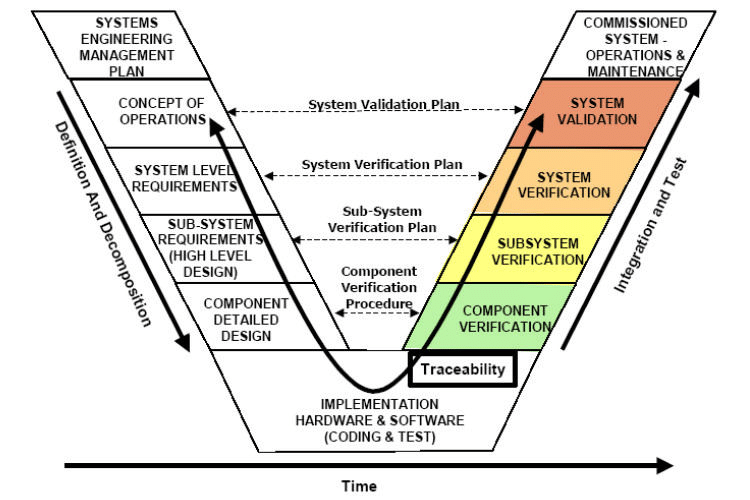
\includegraphics[width=3in]{background/v_diagram.png}
    \labfig{v_method}
\end{figure}

\subsection{Agile Methodology}
The Agile methodology is a relatively new concept introduced in the mid-1990's that provided a radical new method for doing software development.
Instead of working in siloed teams based on a broad set of requirements and a large, expansive Gantt chart, programmers were encouraged to start working together in smaller teams to tackle smaller issues and constantly test and present their progress.
Team leaders would have an easier time managing the smaller teams and workloads, and project managers would have a better way of tracking product progress.
The scrum methodology was also introduced that radically changed the team dynamic and has evolved to improve efficiency in a wide variety of industries \cite{Sutherland:2014}.

The Agile methodology was implemented on the project so that tasking loading remained light and features could be implemented sprint-by-sprint.
The testing recommended by the Agile method meant that products could be more quickly verified and validated against, allowing for quicker iteration.
This meant the project could adapt quickly and provide a framework for new people to start contributing to the project, if necessary.

\section{A Review of the State of the Art} \labsec{literature_review}
Inertial sensing is not a new problem to be solved.
Over the last few decades many solutions have been released with increasingly better performance and efficiency.
The advent of MEMS technology drastically shrunk sensor sizes and made them cheaper to use.
We shall examine two different categories of solutions and compare solutions within those categories.

\subsection{Industrial Solutions} \labsubsec{industrial_solutions}
Industrial solutions are provided by companies to customers that require performance and reliability for their sensors.
They will typically be employed in the industrial robotics or automotive industries and integrated within a larger system.
Thus, they cannot provide standalone services, and do not satisfy the objectives for this thesis.
But, they represent the cutting edge techniques for sensor fusion.
The following solutions also are the ``more affordable'' variants in order to limit the scope of the review.
Even so, each solution is prohibitively expensive and therefore out of the scope of the thesis objectives.

\paragraph*{Sparton AHRS-8} The first industrial sensor to consider is the Sparton AHRS-8 \cite{Sparton} and is one of the cheapest at \$1,350 per unit.
This is an AHRS designed to be interfaced over USB or Serial and uses Sparton's proprietary AdaptNav\textsuperscript{TM} sensor fusion algorithm.
This gives a sub 1-degree accurate measurement of body attitude and heading at a range of temperatures and motions.
However, this sensor lacks GPS/GNSS integration, wireless features, and independent data logging.

\begin{figure}
    \centering
    \caption[Sparton AHRS-8]{Sparton AHRS-8.
    Courtesy of Sparton \cite{Sparton}}
    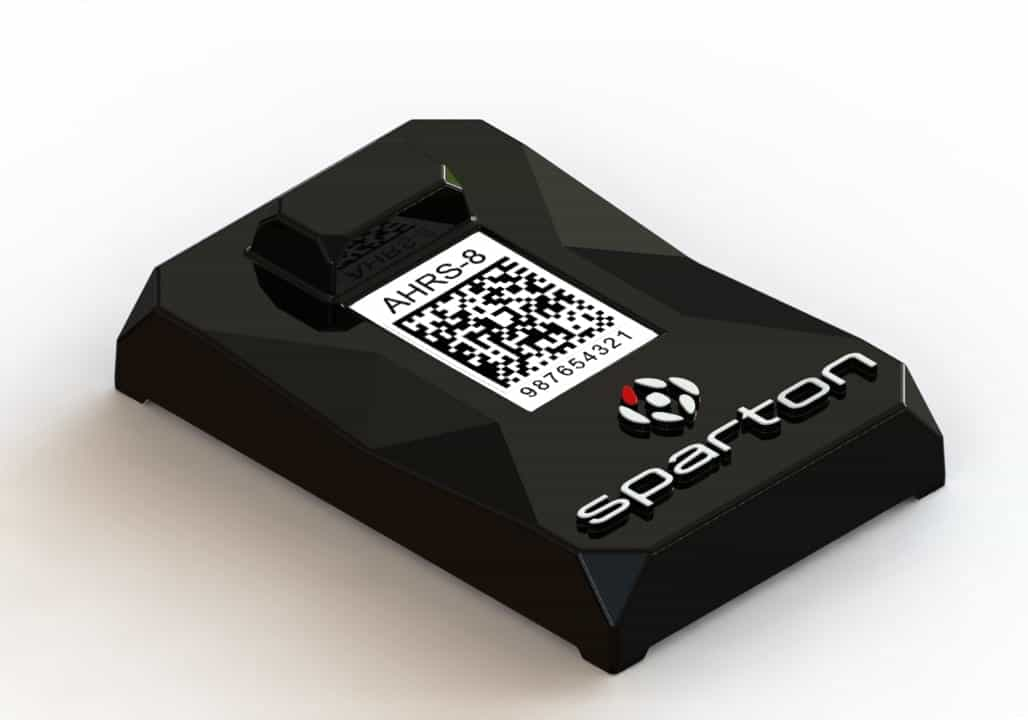
\includegraphics[width=2in]{background/sparton_ahrs8.png}
    \labfig{sparton_ahrs8}
\end{figure}

\paragraph*{Xsens Mti-100} The second sensor to consider comes from the Movella/Xsense corporation and is their MTi-100 IMU \cite{Movella}.
This unit costs \$1,809 and provides an 9-DOF IMU with an RS232, RS422, RS485, UART, and USB output for integration on larger platforms.
Like the Sparton, it runs a proprietary sensor fusion algorithm and does not have GPS/GNSS integration.
But, it does have a software development kit (SDK) provided by the manufacturer to more easily integrate it and tweak settings.
The unit boasts a sub 1-degree accurate orientation estimate over a range of temperatures and motions.

\begin{figure}
    \centering
    \caption[Xsens Mti-100]{The Xsens Mti-100 IMU.
    Courtesy of Movella \cite{Movella}.}
    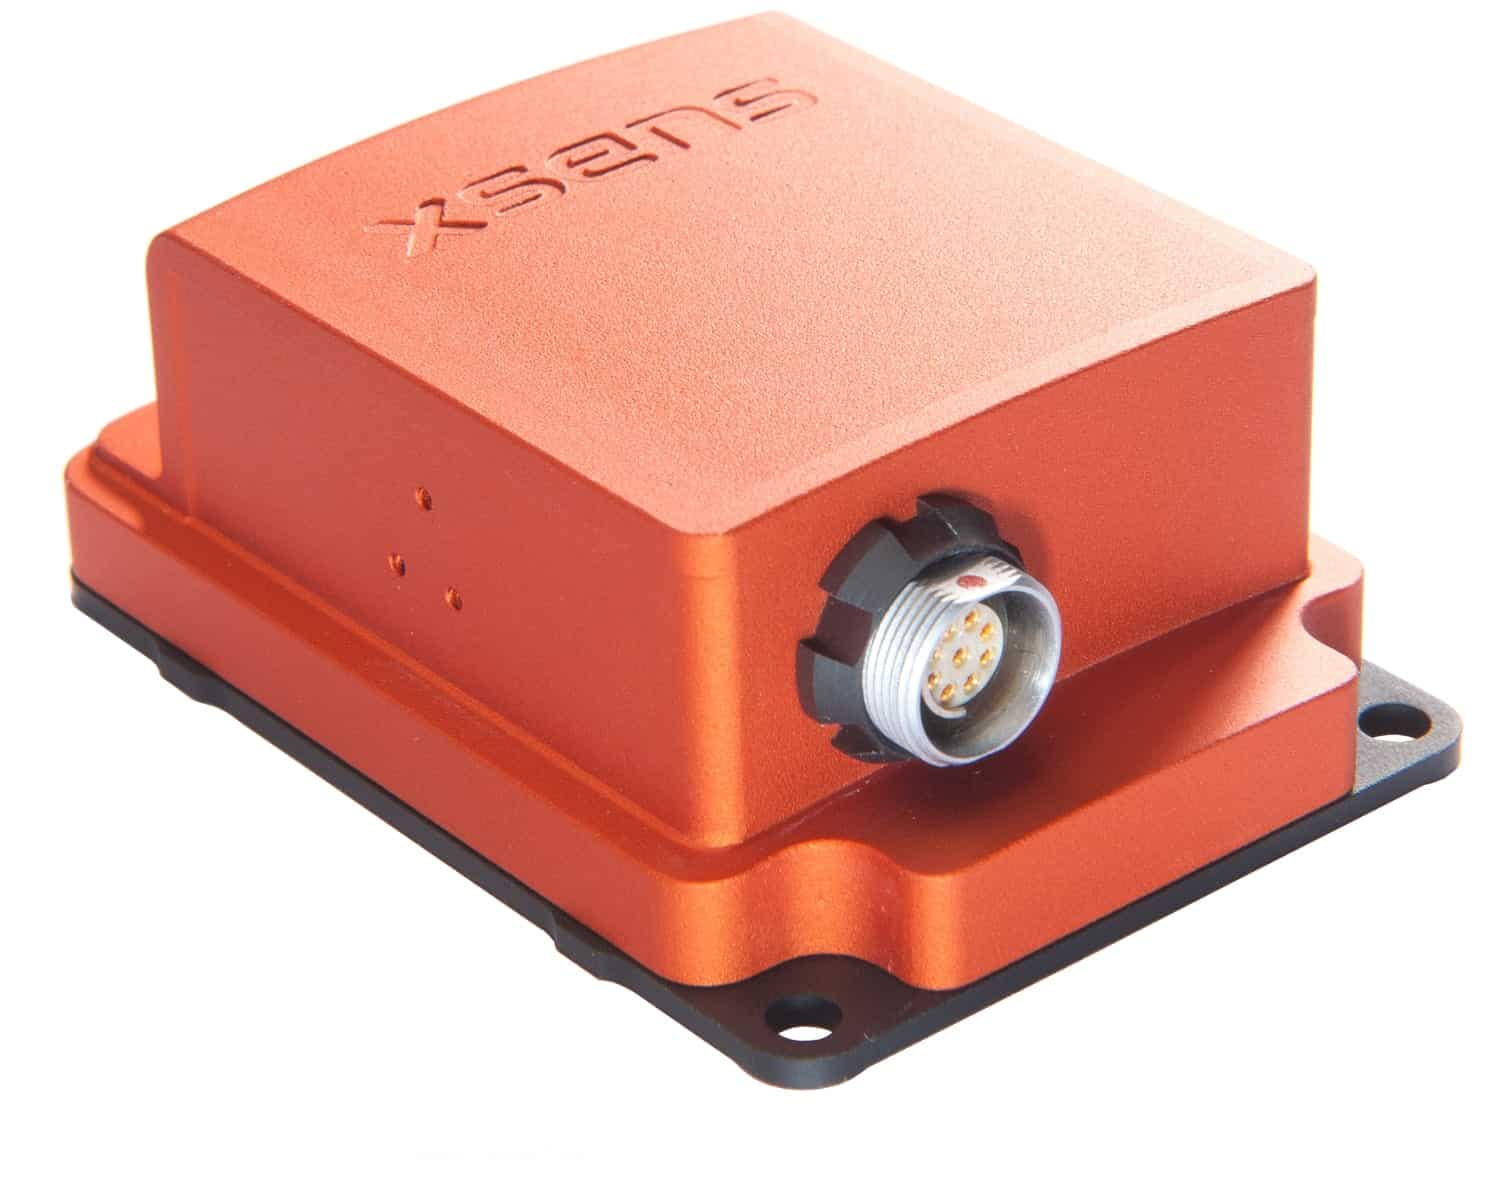
\includegraphics[width=2in]{background/xsens_mti100.png}
    \labfig{xsens_mti100}
\end{figure}

\paragraph*{VectorNav VN-200} From the VectorNav corporation comes the VN-200 AHRS \cite{VectorNav:VN200}.
The unit boasts a \textless 0.2-degree accurate attitude estimation and integrates GPS/GNSS.
However, it relies on a USB or Serial interface and uses closed source and proprietary firmware for sensor fusion.
It also does not have wireless or independent data logging functionality and costs over \$3,000.

\begin{figure}
    \centering
    \caption[VectorNav VN-200]{The VectorNav VN-200 IMU.
    Courtesy of VectorNav \cite{VectorNav:VN200}.}
    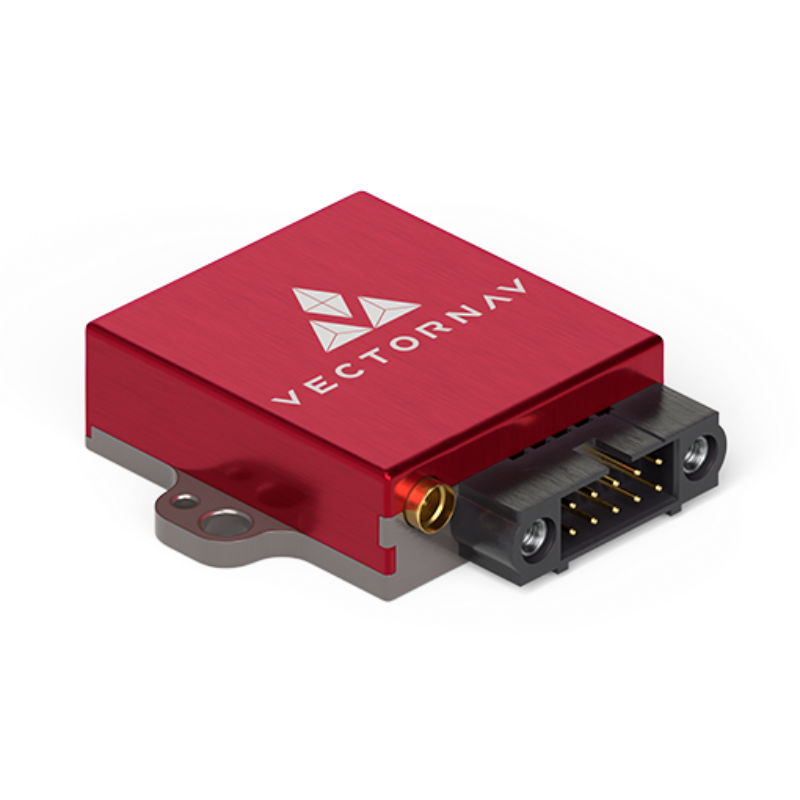
\includegraphics[width=2in]{background/vn200.png}
    \labfig{vn200}
\end{figure}

\paragraph*{SwiftNav Duro} The SwiftNav Duro is a centimeter-accurate GNSS real-time kinematic (RTK) solution that incorporates a high accuracy IMU for inertial navigation \cite{SwiftNav}.
This unit is developed for robotics applications that need a bolt-on solution for autonomous navigation and positioning.
The unit comes in a rugged IP67 enclosure and has multiple interfaces such as USB, Serial, and Ethernet for communications.
However, it does not have wireless or independent data logging functionality.
The firmware is also closed source and it costs \$5,795 per unit.

\begin{figure}
    \centering
    \caption[SwiftNav Duro]{The SwiftNav Duro Inertial.
    Courtesy of SwiftNav \cite{SwiftNav}.}
    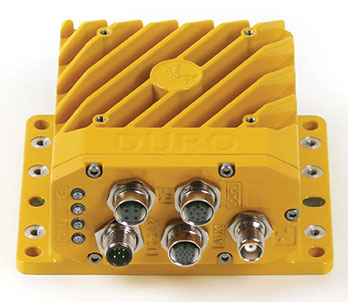
\includegraphics[width=2in]{background/swiftnav_duro.png}
    \labfig{swiftnav_duro}
\end{figure}

\paragraph*{Aceinna INS401} Rounding out the industrial solutions is the Aceinna INS401 which is a rugged centimeter-accurate inertial navigation system (INS) for automotive and industrial autonomous systems \cite{Aceinna}.
The unit is closed source, but provides a developer-friendly SDK and API for integration on a larger platform.
Like its cousins, this unit also does not have wireless connectivity or independent data logging functions, but can communicate over several hard-wired methods.

\begin{figure}
    \centering
    \caption[Aceinna INS401]{The Aceinna INS401.
    Courtesy of Aceinna \cite{Aceinna}.}
    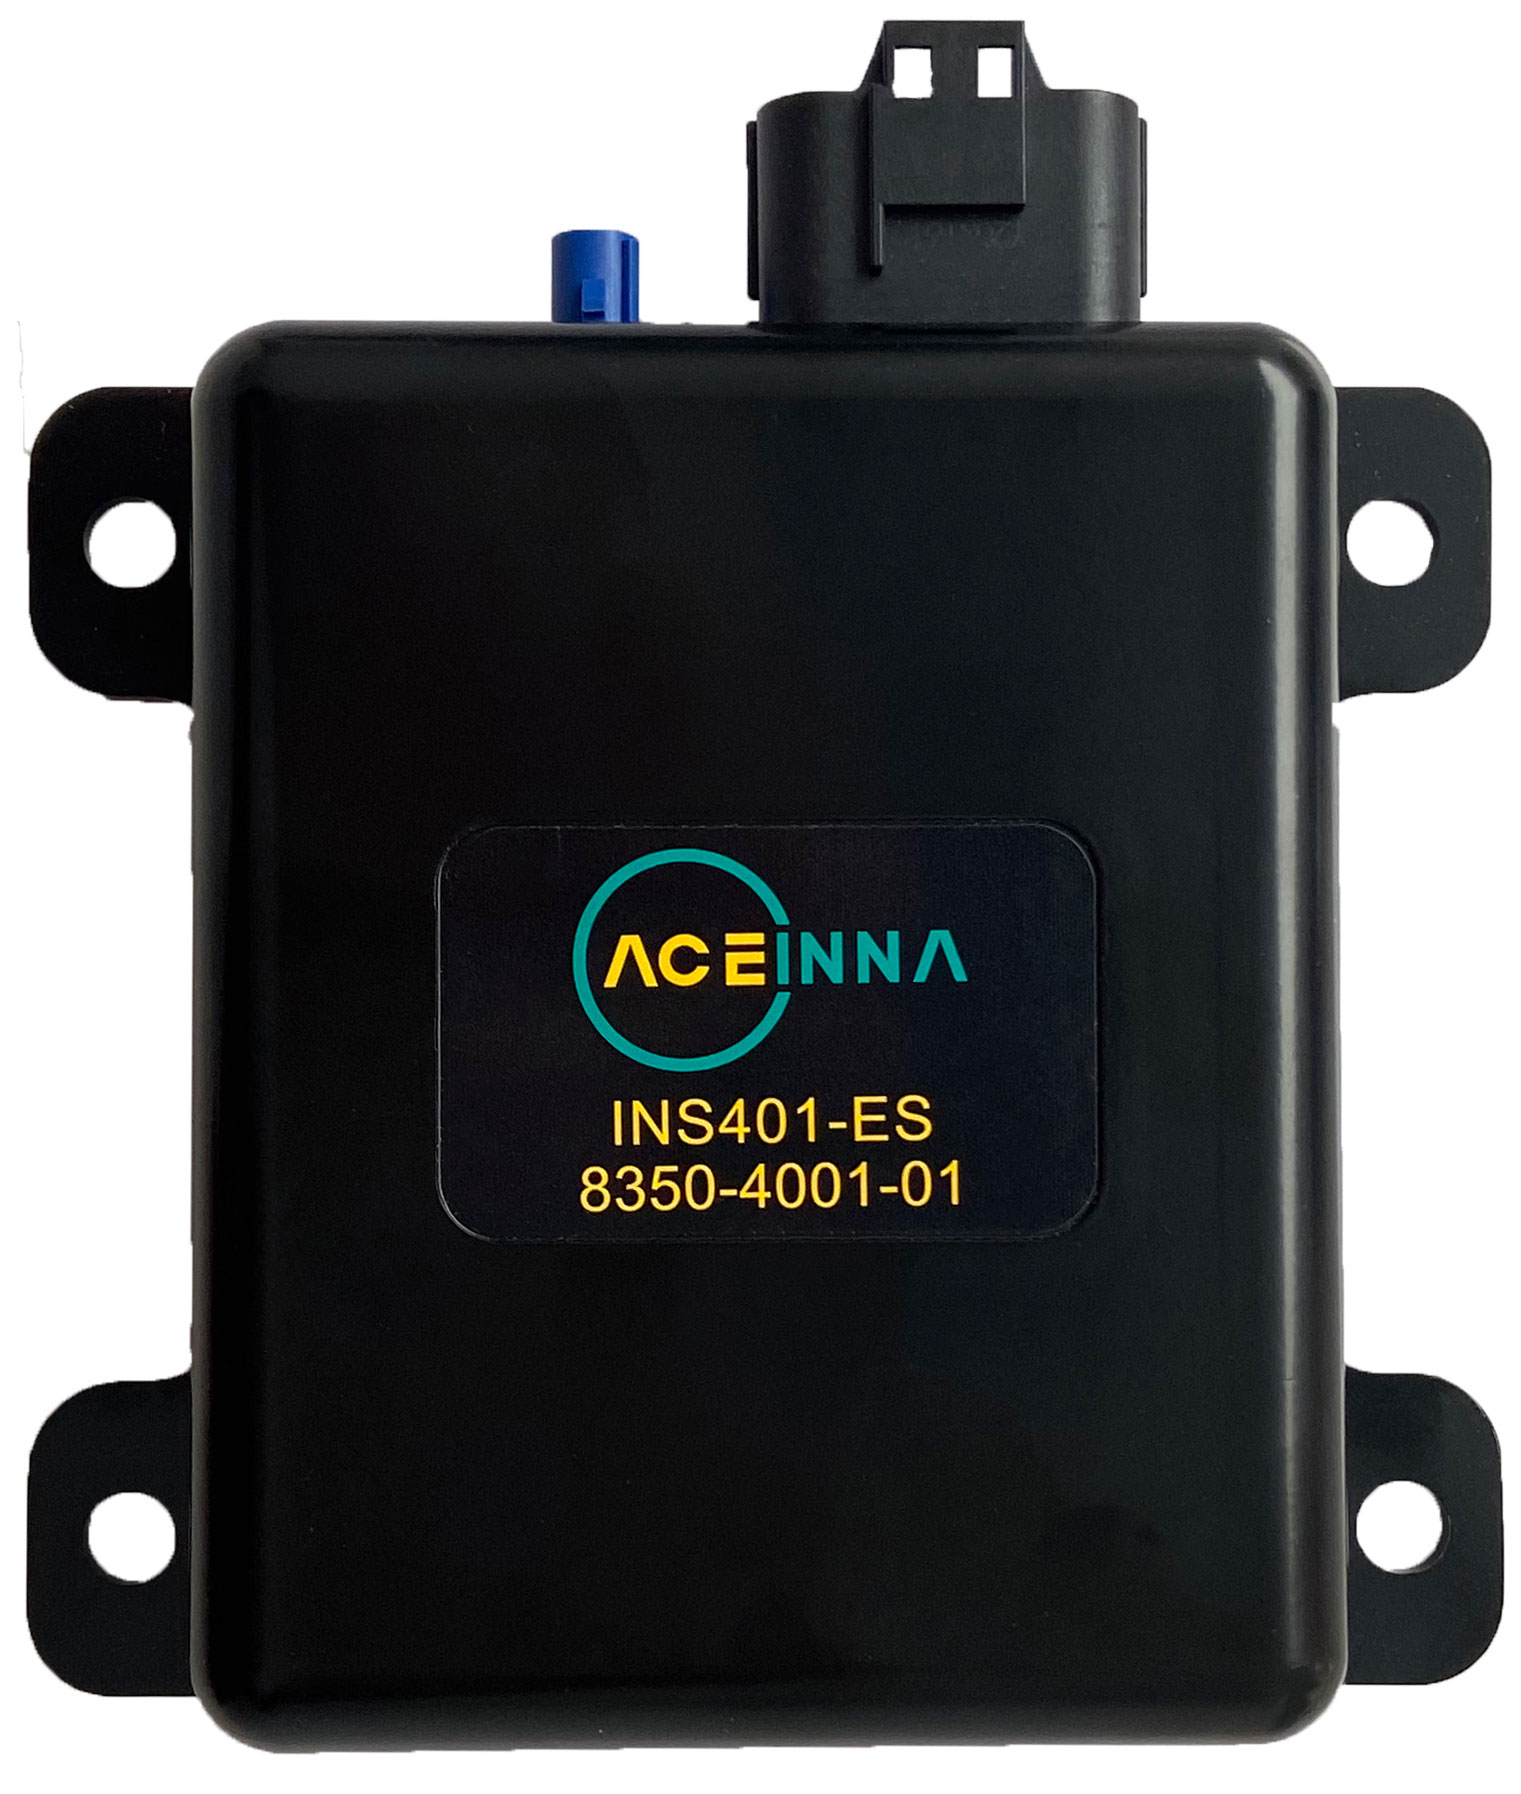
\includegraphics[width=2in]{background/aceinna_ins401.png}
    \labfig{aceinna_ins401}
\end{figure}

\subsection{Hobbyist Solutions}
Stepping down an order of magnitude in pricing and performance are the hobbyist sensors.
These can be purchased by companies such as Adafruit and SparkFun and HobbyBro for tens, if not a couple hundred of dollars per unit, making it much more reasonable for the average consumer to use on their projects.
The hobbyist solutions are much more in line with the objectives of the thesis and should therefore be more carefully considered.

\paragraph*{Kauai Labs NavX2 Micro} The NavX2 micro is derived from the popular NavX board that is routinely used in the First Robotics Competition for high school robotics \cite{KauaiLabs}.
The NavX2 micro shrinks the sensor down into a low SWaP and cost package that utilizes open source software.
This makes it well-suited for its application in hobbyist robotics where even basic inertial navigation is a coveted feature.
The unit costs \$89 and can be integrated onto a larger platform via a USB or Serial interface.
However, it does not have wireless connectivity or independent data logging.
For these reasons, the NavX2 micro will not suit the objectives of this thesis.

\begin{figure}
    \centering
    \caption[Kauai Labs NavX2 Micro]{The Kauai Labs NavX2 Micro.
    Courtesy of Kauai Labs \cite{KauaiLabs}.}
    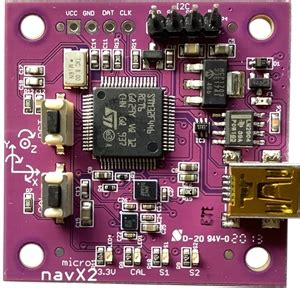
\includegraphics[width=2in]{background/navx2_micro.png}
    \labfig{navx2_micro}
\end{figure}

\paragraph*{SparkFun OpenLog Artemis} The OpenLog Artemis (OLA) is a hobbyist solution offered by SparkFun for \$55 \cite{SparkFun}.
It comes equipped with a 9-DOF IMU, battery integration, a real-time-clock, ADC, and an interface for easily integrating other sensors.
The unit is pre-loaded with firmware that automatically begins logging when it is powered on and the software is open source and can be freely modified.
It even has a BlueTooth interface that can be used to wireless monitor data.
This solution meets the thesis objectives, but the code would have to be modified to perform sensor fusion for orientation estimation and an IP67-rated case would have to designed for it.

\begin{figure}
    \centering
    \caption[SparkFun OpenLog Artemis]{The SparkFun OpenLog Artemis.
    Courtesy of SparkFun \cite{SparkFun}.}
    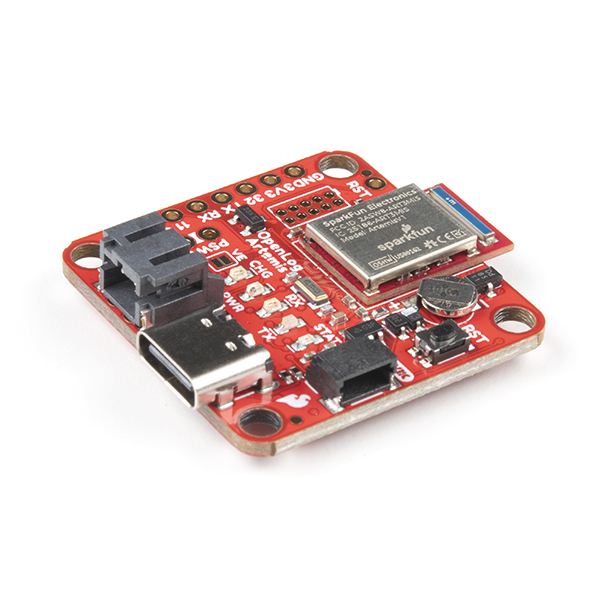
\includegraphics[width=2in]{background/sparkfun_ola.png}
    \labfig{sparkfun_ola}
\end{figure}

\paragraph*{Pixhawk FCU} The Pixhawk Flight Controller Unit (FCU) is designed for hobbyist robotics applications such as drones (UAVs) and remotely operated vehicles \cite{HolyBro}.
It runs a sophisticated open source hardware and software stack that fuses a 9-DOF IMU with GPS data to get position and attitude with a reasonable degree of accuracy.
The sensor fusion is performed with multiple Extended Kalman Filters and can be logged internally to a microSD card.
By using a radio link over the serial bus, data can be wirelessly transmitted to a ground station for monitoring and logging.

This solution fits the objectives of the thesis, however it is overkill for the intended application and the MAVlink interface used to communicate with it is not intuitive.
Because data logging is only meant for post-flight analysis if the vehicle crashes or malfunctions, there are significant limitations on what can be logged or how fast.
For these reasons, the Pixhawk was not considered as a solution for the thesis.

\begin{figure}
    \centering
    \caption[Holybro Pixhawk 6X]{The Holybro Pixhawk 6X FCU.
    Courtesy of Holybro \cite{HolyBro}.}
    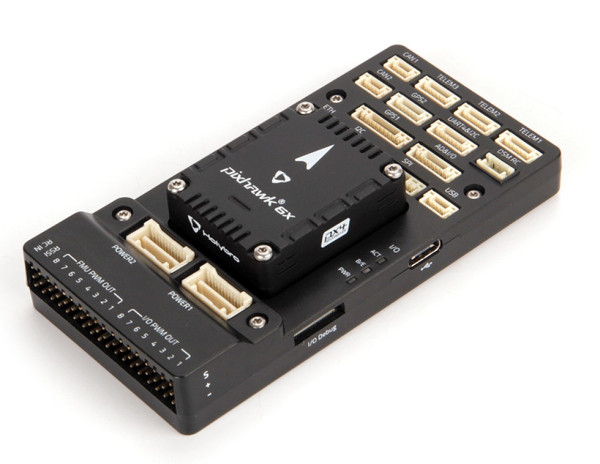
\includegraphics[width=2in]{background/pixhawk_6x.png}
    \labfig{pixhawk_6x}
\end{figure}

\paragraph*{x-io Technologies x-IMU3} Recently released in June 2023, the x-IMU3 has almost the exact same capabilities as the solution presented in this thesis \cite{xioTechnologies}.
This device was designed by the author of the Madgwick algorithm, and is the third iteration of his IMU data loggers.
The x-IMU3 has a very low SWaP and comes in a IP67-rated enclosure with a USB and button interface.
The USB interface can be used to directly link the device and offload files, or it can be used with external peripherals.
Similarly, the x-IMU3 has extensive wireless support and can stream data back to a host application over WiFi (via TCP or UDP) or over BlueTooth.

The x-IMU3 and the thesis were developed independently, but the final products are near to each other in both cost and capability.
In fact, the x-IMU3 was a major influence on the final firmware revision for the thesis and helped implement key features.
The creator, Dr. Sebastian Madgwick, has also been helpful in critiquing the thesis design and offered key insights over multiple interviews \cite{Duffy:2023}.
We shall carefully consider this solution going forward and directly compare it to the thesis product in Chapter \ref{chap:verification_validation}.

\begin{figure}
    \centering
    \caption[x-io Technologies x-IMU3]{The x-io Technologies x-IMU3.
    Courtesy of x-io Technologies \cite{xioTechnologies}.}
    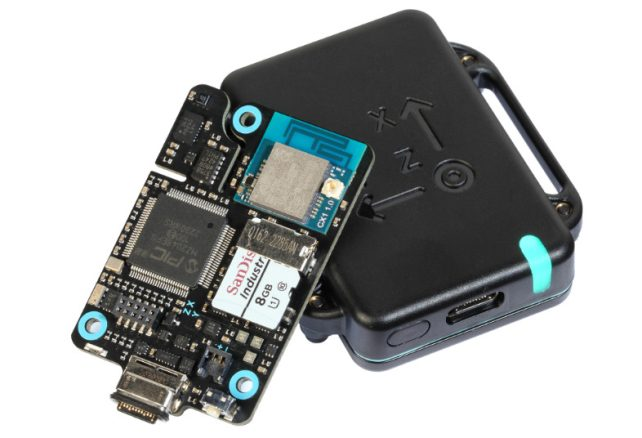
\includegraphics[width=2in]{background/ximu3.png}
    \labfig{ximu3}
\end{figure}